\chapter{Luminometer Calibration}
\label{ch3}


Accurate measurement of the luminosity delivered to the CMS experiment by the LHC is essential for various reasons. Online, the luminosity measurement provides feedback on the performance of both the LHC and CMS during operations, including monitoring trigger rates. In offline analysis, it is a critical component for measuring the cross-section of observed processes \cite{pas_18}.  

The determination of \( \sigma_{\text{vis}} \) is performed using the van der Meer (vdM) method, which is carried out through a specialized scan program using a dedicated LHC machine setup. This chapter describes this procedure and the final calibration of the PCC luminometer.


\section{van der Meer (vdM) method}
\label{vdM method}

The instantaneous luminosity for a single colliding bunch pair at head-on, seperated by $(\Delta x, \Delta y)$ is described by:


\begin{equation}
\label{eq:lumidef}
\mathcal{L} (\Delta x, \Delta y) = N_1 N_2 f\int_{-\infty}^{\infty}\rho_1(x,y)\rho_2(x+\Delta x,y+\Delta y) \,dx\,dy
\end{equation}


where $N_1$ and $N_2$ are the numbers of protons in the two colliding bunches, respectively, $f = 11245.6$ Hz is the revolution frequency of the LHC, and $\rho_i$ denotes the proton density distribution of the $i^{\text{th}}$ bunch. While the bunch populations can be measured with good precision, accurately determining the proton density profiles entering Equation~\ref{eq:lumidef} is more challenging. The van der Meer (vdM) scan method, used by LHC experiments, enables the measurement of the integral over the bunch proton densities appearing in Equation~\ref{eq:lumidef}.

For the vdM method to be applicable, it is assumed that the proton density distributions of the two bunches factorize in the transverse directions $x$ and $y$:

\begin{equation}
\label{eq:fact}
\int_{-\infty}^{\infty} \rho_1(x,y) \rho_2(x+\Delta x, y+\Delta y) \, dx \, dy = \int_{-\infty}^{\infty} \rho_1(x) \rho_2(x+\Delta x) \, dx  \times  \int_{-\infty}^{\infty} \rho_1(y) \rho_2(y+\Delta y) \, dy.
\end{equation}


Both sides of Equation~\ref{eq:lumidef} can then be integrated independently over $\Delta x$ and $\Delta y$, while keeping the other separation fixed. This yields:

\begin{equation}
\label{eq:evaldense}
N_1 N_2 f \int_{-\infty}^{\infty} \rho_1(y)\rho_2(y+\Delta y_0) \,dy = \int_{-\infty}^{\infty} \mathcal{L}(\Delta x, \Delta y_0) \,d(\Delta x),
\end{equation}

and therefore,

\begin{equation}
\label{eq:evaldense2}
\int_{-\infty}^{\infty} \rho_1(x)\rho_2(x+\Delta x_0) \,dx = \frac{\mathcal{L} (\Delta x_0, \Delta y_0)}{\int_{-\infty}^{\infty} \mathcal{L}(\Delta x, \Delta y_0) \,d(\Delta x)}.
\end{equation}


Likewise for $y$. Experimentally, the integration over $\Delta x$ and $\Delta y$ is implemented by scanning the two beams against each other, and the integral on the right-hand side of Equation~\ref{eq:evaldense} is evaluated by measuring the luminometer rate as a function of the beam-beam separation. Equation~\ref{eq:lumidef} then becomes, after replacing the beam overlap integrals in $x$ and $y$ according to Equation~\ref{eq:evaldense2}, for a particular head-on working point $(\Delta x_0, \Delta y_0)$:

\begin{equation}
\label{eq:lumidefVdM}
\mathcal{L} (\Delta x_0, \Delta y_0) = N_1 N_2 f  \frac{R (\Delta x_0, \Delta y_0) R (\Delta x_0, \Delta y_0)}{\int_{-\infty}^{\infty} R (\Delta x, \Delta y_0) \,d(\Delta x) \int_{-\infty}^{\infty} R(\Delta x_0, \Delta y) \,d(\Delta y)},
\end{equation}

where the luminosity is replaced by the measurable rate $R(\Delta x, \Delta y)$ when  the two beams are seperated by ($\Delta x$,$\Delta y$). Since the Van der Meer procedure is a physical convolution of the two beams, it is common to re-write the beam overlap width $\Sigma_x$ (and similarly $\Sigma_y$) as:


\begin{equation}
\label{eq:capsigma}
\Sigma_x = \frac{1}{\sqrt{2\pi}}\frac{\int_{-\infty}^{\infty} R_x{} (\Delta) d(\Delta)}{R_{x}(0)},
\end{equation}

giving

\begin{equation}
\label{eq:lumidefVdMcSig}
\mathcal{L}_{inst} =\frac{N_1 N_2 f}{2\pi\Sigma_x \Sigma_y},
\end{equation}

such that the final formula used to measure the visible cross sections is

\begin{equation}
\label{eq:sigVisX}
 \sigma_{vis}=\frac{2\pi\Sigma_x \Sigma_y R(0,0)}{N_1 N_2 f}.
\end{equation}


In practice, while all quantities on the right-hand side of Equation \ref{eq:sigVisX}, such as the beam currents $N_{1,2}$ and the orbit frequency $f$, are well determined, the overlap integrals $\Sigma_x$ and $\Sigma_y$ cannot be directly measured. Instead, they are extracted from fits to the scan curves obtained from the luminometer rate measurements during the vdM scans. The vdM method involves a specific machine setup (vdM program) that enables the determination of the beam overlap integrals. This is achieved by varying the transverse separation between the beams and recording the resulting interaction rates, which typically yield beam density profiles approximated by normal distributions.

The measured rate, denoted by $R(\Delta x_0, \Delta y_0)$, is defined as the average value of the peak rates obtained during the $x$- and $y$-scans. Although the beam widths are identical for all luminometers, the peaks of the scan curves are specific to each luminometer.

Figure \ref{vdm_sketch} depicts a schematic of the beam positions during vdM scans in the $x$ and $y$ planes, along with the detector rate as a function of beam separation  \cite{pas_18}.

\begin{center}
  \begin{figure}[h]
    \centering
    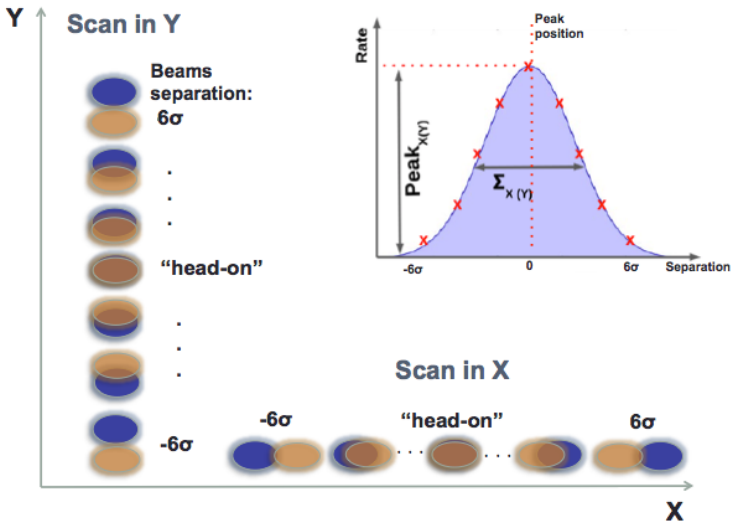
\includegraphics[scale=.40]{Chapter3/vdm_sketch.png}
    \caption[Sketch of a vdM scan in $x$ and $y$ directions and example of fitting resulting rates]{ The sketch of a vdM scan in $x$ and $y$ planes. The indent sketch is an example of the fit of the resulting rates \cite{vdM_sketch}.}
    \label{vdm_sketch}
  \end{figure}
\end{center}


\section{vdM program and Scan types}
\label{vdM program and Scan types}

Each year, the vdM scan program for the CMS experiment is conducted during specific LHC fills using a dedicated setup. The LHC filling schemes are designed with a specific number of bunch pairs at the CMS interaction point (IP5), for the especific case of 2017 an 2018 was at a proton-proton collision energy of \(\sqrt{s} = 13\) TeV. These scans play a crucial role in the precise determination of the luminosity by measuring the transverse beam profiles and overlap integral.  

To minimize long-range beam-beam effects and detector background (afterglow), the bunches are arranged in a way that optimizes the measurement conditions. During these special fills, the beams are systematically displaced in the transverse plane, allowing for a detailed study of beam dynamics and interaction rates. Various types of scan pairs with different characteristics were conducted to refine the accuracy of the luminosity determination.  

Each scan pair consisted of two scans in the transverse \(x\) and \(y\) planes. These included standard vdM scans, emittance scans, beam imaging scans, offset scans, and length scale calibration scans, each serving a specific purpose in the calibracion and luminosity measurement process. A detailed description of each scan is provided below.  

\noindent \textbf{Standard vdM}: used specifically to compute $\sigma_{vis}$, in this scan the two beams are separated by $6\sigma_{b} \thickapprox 578\mu m$, where $\sigma_{b}$ represents the transverse bunch size. and scanned across each other in a se quence of 25 steps with 30 seconds per step with a step size of $0.5\sigma_{b} \thickapprox 48 \mu m$ in either the horizontal (x) or vertical (y) direction.\\

\noindent \textbf{Emittance}: same procedure as the standard vdM scans except the maximum separation (2.5 − $4 \sigma_{b}$), the number of steps (7 or 9) and the time per step (10 seconds) are smaller, so that the scan takes a shorter time. These type of scans are also performed in physics conditions as discussed in Section.\\
 
\noindent \textbf{Beam imaging}: in these scans, one beam (beam 1 and beam 2, respectively) is kept fixed at its nominal head-on position, while the other beam is separated and scanned in 19 steps, each step lasts 46 seconds and covers a range from $-4.5\sigma_{b}$ to $+4.5\sigma_{b} \thickapprox 433 \mu m$. These scans were developed for studies on beam shapes, estimating the uncertainty caused by the correction called $x$-$y$ non-factorization described in the next chapter. BI scans are also analyzed as traditional vdM scans and used to compute of $\sigma_{vis}$.\\
 
\noindent \textbf{Constant-Separation Length Scale}: during this scan the two beams are separated by $\sqrt{2} \sigma_{b} \thickapprox 106 \mu m$ (approximately equal to $1 \Sigma_{b}$) and moved together in steps of $1\sigma_{b}$ forward and backward in five steps each, for a total of 10 steps with 70 seconds per step.\\

\noindent \textbf{Variable-Separation length scale}: one beam (starting with beam 1) is moved to $-2.5\sigma_{b}$ and then a three-point scan is performed with the other beam (starting with beam 2) at arelative position of $+-1.25\sigma_{b}$, 0, and $+1.25\sigma_{b}$. The position of the first beam is then stepped in five steps to $+2.5\sigma_{b}$, repeating the three-point scan (“miniscan”) at each step. This procedure is repeated four times, with two directions for each of the two beams. Each scan point has a duration of about 46 s.
 
The two types of Length scale are pecial scan designed to apply a correction to the results of  $\sigma_{vis}$ obtained from the vdM scan program, this correction will be described further in this section.\\
 
\noindent \textbf{Offset}: same procedure as the standard vdM scans except that the beams are separated by  range from $-3\sigma_{b}$ to $+3\sigma_{b}$ in the non-scanning direction.\\ 
 
\noindent \textbf{Super Separation}: this type of scan is performed for background estimation. In this scan, the two beams are separated by a distance of \(6\sigma_{b}\) for 5 minutes. At this distance, the beam overlap is minimal, and the contribution from collisions is negligible.  
There can be more than one Super Separation scan per scan program, this is useful to understanding the behavior of the background throughout the year and for subtracting it accordingly.

The data collected from these scans provide the essential input for luminosity calibration, which is critical for cross-section measurements and precision physics analyses at the LHC.
 
\subsection{2017 vdM scan program}
\label{2017 vdM scan program}

The 2017 vdM scan program was performed during LHC fill 6016 on 28 July 2017, at a center-of-mass energy of 13 TeV. The LHC filling scheme included 32 colliding bunch pairs at the CMS interaction point (IP5). In the special case of PCC, to ensure a dataset with a high event count at large beam separations, CMS gated the zero-bias triggers on 5 bunch pairs (BCIDs 41, 281, 872, 1783, and 2063) and recorded events at a total rate of 18 kHz.  

The bunch intensities were approximately \(9 \times 10^{10}\) protons per filled bunch, resulting in a total beam intensity of approximately \(4.5 \times 10^{12}\) protons per beam. The total beam intensities were measured with the DC Current Transformers (DCCT) ~\citep{LHC_DCCT_calibration}.  The beam orbit was monitored using two systems: the DOROS beam position monitors (BPMs) ~\citep{BPM__electronics}, located near IP5, and the arc BPMs, located in the LHC arcs adjacent to CMS.  

The vdM scan program consisted of a total of eight orthogonal (x-y) scan pairs. It started with a short emittance scan, em1. Four scans were standard vdM scans: vdM1 (2), vdM3 (6), and vdM4 (11). These scans were performed first in the x direction and then in the y direction. The intermediate scan, vdM2 (3), was performed first in the y direction and then in the x direction. This was done to check reproducibility.  

Two scan pairs of beam imaging scans were performed, with beam 1 and beam 2 scanning. Pairs Im1 and Im2 corresponded to scans 4 and 5, respectively. Scan pair 7 was an offset scan (off) performed just after vdM3, but it is not used in this analysis.  

A length scale calibration (LSC) program was performed at the end of the vdM program using two different LS methods. The first method was the constant-separation scan (cLS), performed as scan 8 in this program. This type of scan had been previously used in the 2015–2016 publication  ~\citep{lumi_precise_2015_2016} for the CMS length scale calibration.

The second method consisted of variable-separation scans, vLS1 and vLS2, which were scans 9 and 10, respectively, in the LS program. This method was used for the first time in 2017, following the scan protocol originally developed by ATLAS.  

The top of Figure~\ref{BeamPosition_2017} shows the beam positions for the two beams in the x and y directions as measured by the DOROS BPMs during the 2017 scan program, showing the four regular scan pairs, the two beam imaging scan pairs, the offset scan pair, and the two length scale scan programs, with the abbreviations used for the scans introduced.  

%\begin{center}
  \begin{figure}[h]
    \hspace{-.4cm}
    %\centering
    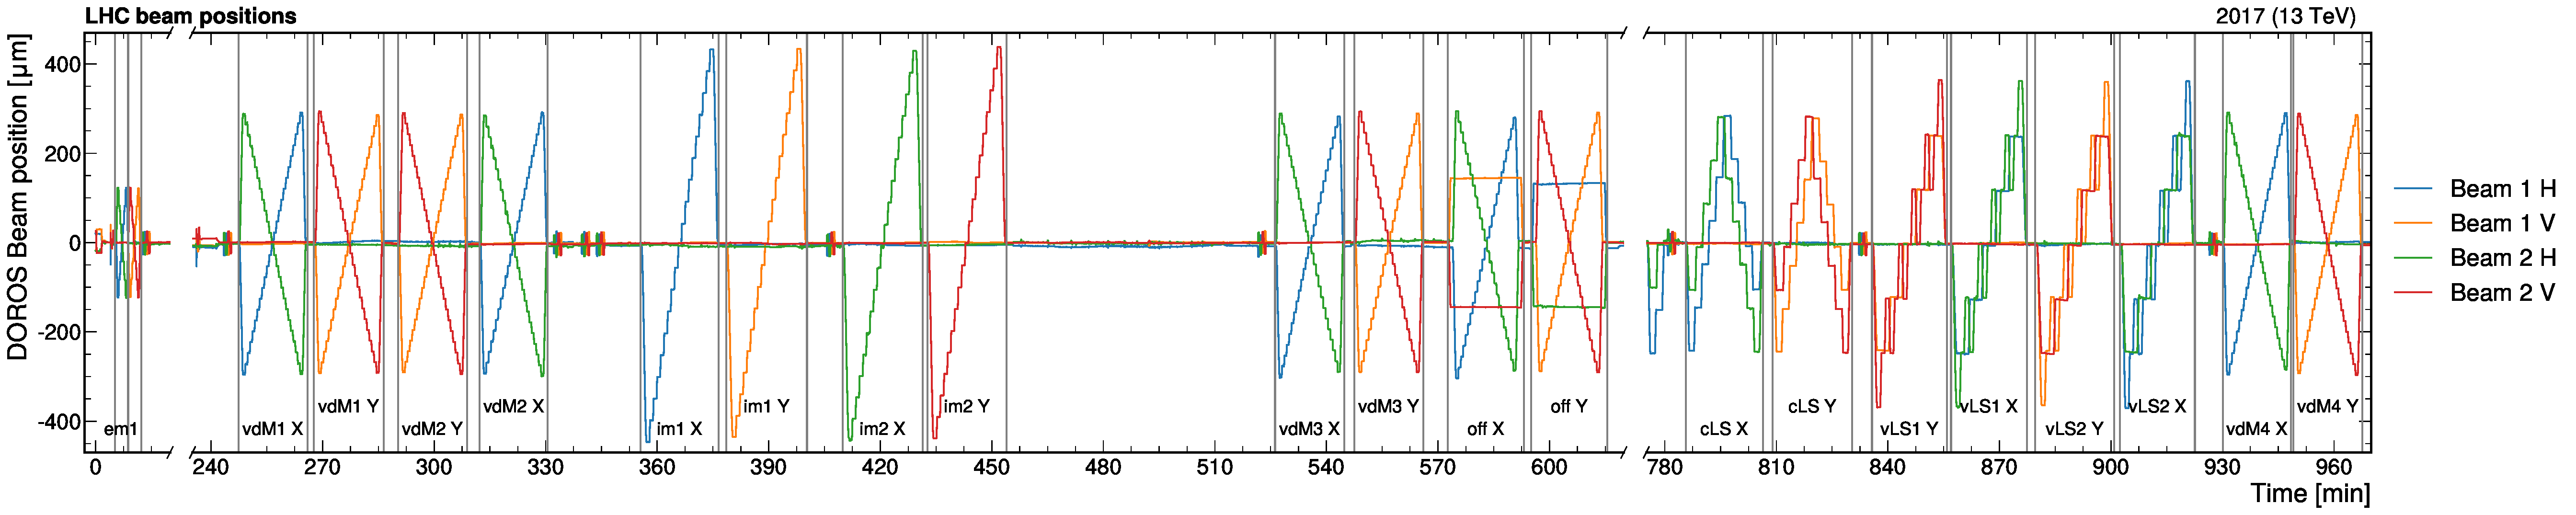
\includegraphics[scale=.17]{Chapter3/BeamPosition/doros_vs_time_6016.pdf}
    \caption[Beam Position in vdM scan 2017]{ Vertical (V) and horizontal (H) beam positions as a function of time measured by the DOROS beam position monitors during LHC fill 6016. The orbit is averaged over the bunches and monitored throughout the scan program with 1 second time granularity. The individual scans are delimited by the vertical lines. Each scan pair consists of two scans orthogonal to each other and labelled with the abbreviation of the specific scan type}
    \label{BeamPosition_2017}
  \end{figure}
%\end{center}


\subsection{2018 vdM scan program}
\label{2018 vdM scan program}

The 2018 vdM scan program was conducted during LHC fill 6868 from June 30 to July 1, 2018, at a center-of-mass energy of 13 TeV. The LHC filling scheme included 124 colliding bunch pairs at the CMS interaction point (IP5). For the special case of PCC, to ensure a dataset with a high event count at large beam separations, CMS gated the zero-bias triggers on 5 bunch pairs (BCIDs 265, 865, 1780, 2192, and 3380) and recorded events at a total rate of 27 kHz.  

In this year the bunch intensities were approximately \(7-9 \times 10^{10}\) protons per filled bunch, resulting in a total beam intensity of approximately \(4.5 \times 10^{13}\) protons per beam. The beam intensities and the beam orbit were measured and monitored in the same way as in 2017.

The vdM scan program was conducted in two parts due to an alarm and a power cut. The first part consisted of a total of five x-y scan pairs.First, two short emittance scans, em1 (1) and em2 (2), were conducted, respectively. Then, a standard vdM scan pair, vdM1 (3), was performed, followed by an offset scan, off1 (4). Finally, a pair of beam imaging scans, BI1 (5) and BI2 (6), were onducted, but only the first was completed before the alarm interrupted the program.  

The second part of the program was conducted approximately 7.5 hours later and consisted of 12 scan pairs. Scan pair em3 (6) was a short emittance scan, followed by beam imaging scan pairs Im3 (7) and Im4 (8), then an offset scan pair, off2 (9), and finally two standard vdM scan pairs, vdM2 (10) and vdM3 (11). The latter two allowed us to test the reproducibility of the measurement.  

A length scale calibration program was performed after vdM3 using constant-separation and variable-separation scan pairs: cLS (12), vLS1 (13), and vLS2 (14). Finally, a standard vdM scan pair, vdM4 (15), and two short emittance scan pairs, em4 (16) and em5 (17), concluded the program.  

In each scan pair, the scan was performed first in the x direction and then in the y direction, with the exception of the variable vLS calibration scan pairs, which were performed in the opposite order.  

Additionally, two Super Separation periods were conducted. The first, SS1, took place right after vdM3 was completed, and the second, SS2, followed vdM4. These periods are not included in the final count of scan pairs since they only involve separating the beams in a single direction. They are used for the final estimation of background noise, which will be subtracted in the final analysis. The details of these periods will be discussed in the following chapter.  

The bottom of Figure~\ref{BeamPosition_2018} shows the beam positions for the two beams in the x and y directions as measured by the DOROS BPMs during the 2018 scan program, showing the 17 scan pairs.4 regular scan pairs, the 3 beam imaging scan pairs, the 2 offset scan pair, and the 3 length scales, the emitance scan a the 2 Superseparation periods with the corrsponding abbreviations used.  


%[15] M. Gasior, J. Olexa, and R. Steinhagen, “BPM electronics based on compensated diode detectors — results from development systems”, Conf. Proc. C1204151 (2012) 44.
%[7] C. Barschel et al., “Results of the LHC DCCT calibration studies”, Technical Report 2349 CERN-ATS-Note-2012-026 PERF, 2012.


%\begin{center}
  \begin{figure}[h]
  \hspace{-0.4cm}
    %\centering
    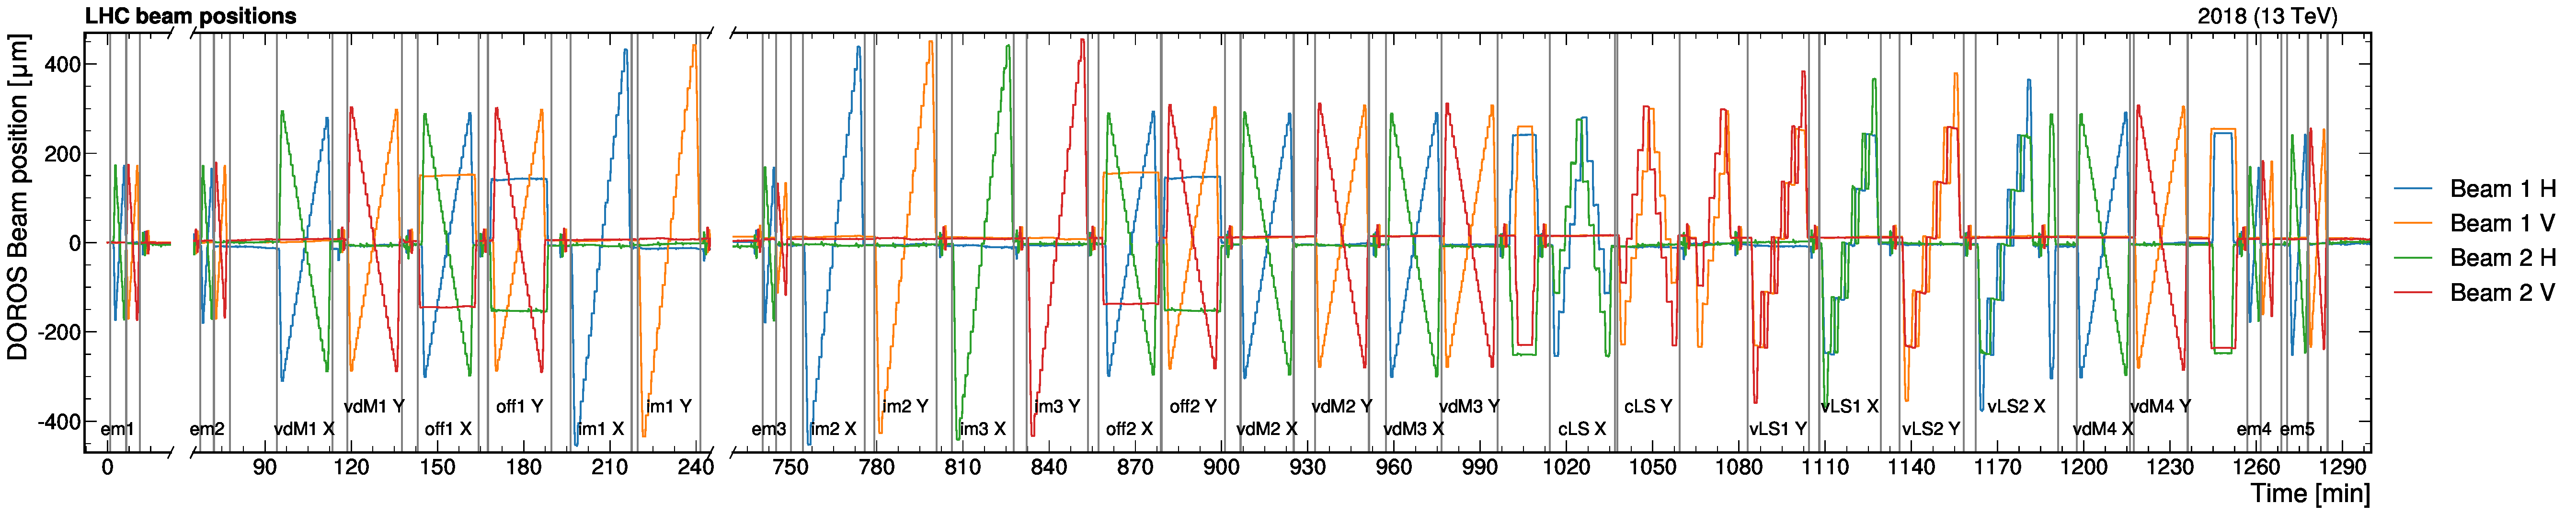
\includegraphics[scale=.17]{Chapter3/BeamPosition/doros_vs_time_6868.pdf}
    \caption[Beam Position in vdM scan 2017]{Vertical (V) and horizontal (H) beam positions as a function of time measured by the DOROS beam position monitors during LHC fill 6868. The orbit is averaged over the bunches and monitored throughout the scan program with 1 second time granularity. The individual scans are delimited by the vertical lines. Each scan pair consists of two scans orthogonal to each other and labelled with the abbreviation of the specific scan type.}
    \label{BeamPosition_2018}
  \end{figure}
%\end{center}



\section{Data acquisition and processing}
\label{data}

As specified in the vdM program, achieving high statistical precision for each colliding bunch pair is constrained by system trigger bandwidth limitations, which prevent the use of all bunches. To address this, CMS implemented zero-bias triggers (defined in Section \ref{Luminometers}) on only five Bunch Crossing IDs (BCIDs): 41, 281, 872, 1783, and 2063 for 2017, and 265, 865, 1780, 2192, and 3380 for 2018.\\

The data is recorded randomly at the highest possible rate of 18 kHz for 2017 and 27 kHz  for 2018, using the High-Level Trigger (HLT) through the CMS Data Acquisition (DAQ) system. Due to the weight of the events, eight different streams per year are required to store the full dataset. These datasets are saved in CMS RAW format, containing event-by-event and bunch-by-bunch information, including the amount of charge deposited in each pixel.\\ 

The data is then reprocessed by the CMS collaboration to enable cluster reconstruction, resulting in datasets (ALCARECO version) that contain a collection of modules and their number of clusters per event. The data is in CMSSW format. These datasets will serve as the starting point for our own data reprocessing and analysis.\\

The ALCARECO samples are processed using CMSSW software to extract clusters per module. Due to the large size of the datasets, all the datasets were sent for reprocessing through The Worldwide LHC Computing Grid (WLCG). During this process, the required cluster counts were obtained and saved in a dataset with ROOT format (a data analysis framework used in high-energy physics) \cite{ROOT}. This format uses TTrees and TBranches, which are containers that organize and store information hierarchically.  
The data is stored per event and includes details such as the number of pixel clusters, the BCID, module identifiers, the run number, the number of lumisections (LS = 23 s), the number of luminible (LN = 0.32 s), and the time at which the event occurred.
\\

The vdM framework (vdMFW), developed by the collaboration for the vdM calibration analysis and the extraction of \( \sigma_{\text{vis}} \), has limitations in its performance. As a result, in previous analisys, not all available statistics were used for PCC detector. To improve this and maintain full statistical precision, rates were stored every 1.32 seconds (NB4), which corresponds to 4 LN. This was achieved by averaging the clusters and the number of events that fall within this time span. During this process, bad modules were removed from the analysis (a detailed discussion of the module veto criteria appears in the following chapter). In this phase, the information is merged into a single file using a hierarchical data format (HDF5) \cite{HD5}, which organizes the data into tables. This final format constitutes a requirement for the vdMFW. The entire processing chain was executed on LxBatch, CERN's computing cluster infrastructure.\\

Finally, the HDF5 file containing the rates collected during the vdM scans is analyzed using the vdMFW. The vdMFW extracts the necessary information using its analysis tools, while subtracting the background and applying several corrections to the measured rates (described in sections \ref{bkg} and \ref{bbcorrections}). During the processing, the vdMFW generates the final information and plots, which contain the normalized rates ($R/N_{1}N_{2}$) and beam position. A fit is then performed on the data points of the scan to extract $\Sigma_{x,y}$ and peak values, which are used to compute $\sigma_{\text{vis}}$ for all the bunches in the scan.


\section{Background estimation}
\label{bkg}


To perform accurate fitting of the data, it is necessary to take into account the following background contributions to the PCC rates. These contributions are estimated independently during the Super Separation (SS) periods discussed in the previous section. Three primary sources of beam-induced background should be considered:

\begin{itemize}

\item Beam Halo (BH): This component occurs when the secondary particles reach the experimental cavern from the LHC tunnel. The primary beam halo is  the population of beam protons characterized by offsets in the transverse coordinates, travelling in  radial amplitude around the beam axis and being captured mostly by the LHC collimation system. In every step of the multi-stage cleaning system of the LHC, more halo particles are captured but also secondary showers are created by the interaction of the beam particles with the collimator material. The largest contribution of the  beam halo to the background consist of secondary particles  that stem from the interactions of the beam halo particles at the tertiary collimators and arrive in large radius into the CMS cavern \cite{beam_halo}.

\item  Beam Gas Inelastic (BGI): This component arises from all inelastic interactions between primary beam protons and residual gas in the beam pipe. The interaction rate is largely influenced by the quality of the vacuum in the various beam line elements upstream of CMS, so the source of this contribution is distributed throughout the long straight section \cite{bkg_source}.

\item Beam Gas Elastic (BGE): The elastic beam gas contribution is made up of all the coherent and quasi-elastic, nuclear elastic, and Coulomb scattering for multi-turn beam-gas interactions around the ring.  \cite{bkg_source}.

\end{itemize}


As mentioned in the previous chapter, the background analysis requires a special scan known as the Super Separation Period. However, for the 2017 vdM calibration program, no Super Separation Period was conducted, and therefore, no data was obtained for the standard analysis. Therefore, a different strategy was implemented: a detailed analysis of the PCC rate tails from the vdM scans. This approach examines PCC rates at the most separated beam positions (i.e., the last points in the tails) to evaluate background levels for each BCID over time. While the standard method averages values across different BCIDs, significant variations were observed among them. Consequently, a different background value was assigned to each BCID used in this year (41, 281, 872, 1783 and 2063). Fig.~\ref{fig:SS_rates} shows the study in which the tail rates were extracted for the four standard vdM scans conducted in 2017. The average rate for each BCID is taken as the measured background to be subtracted, while the standard deviation of these values is used as the error.


\begin{figure}[h]
    \centering
    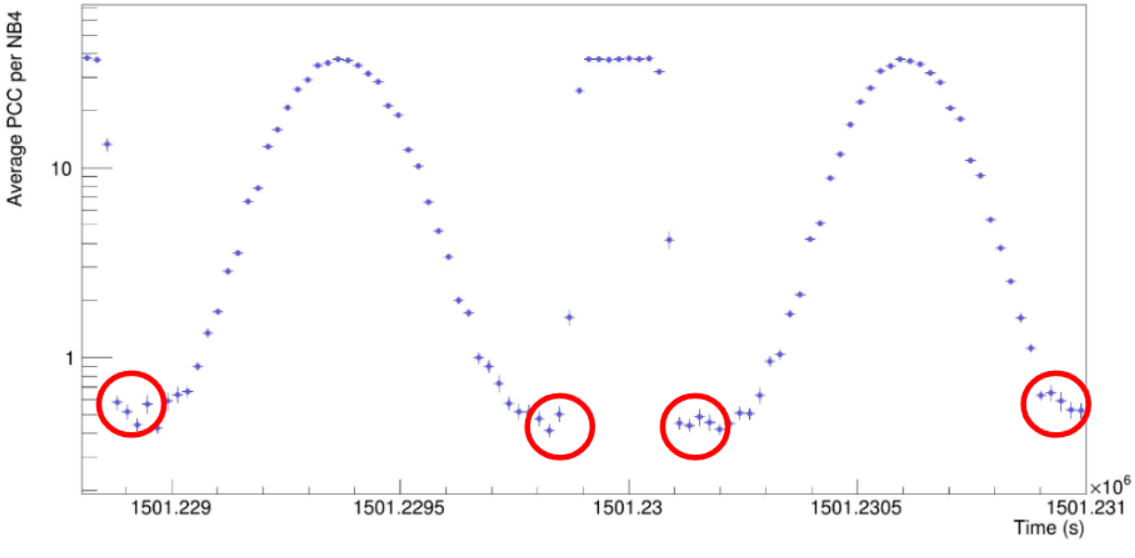
\includegraphics[width=0.44\textwidth,height=0.27\textwidth]{Chapter4/scan_rates.png}
    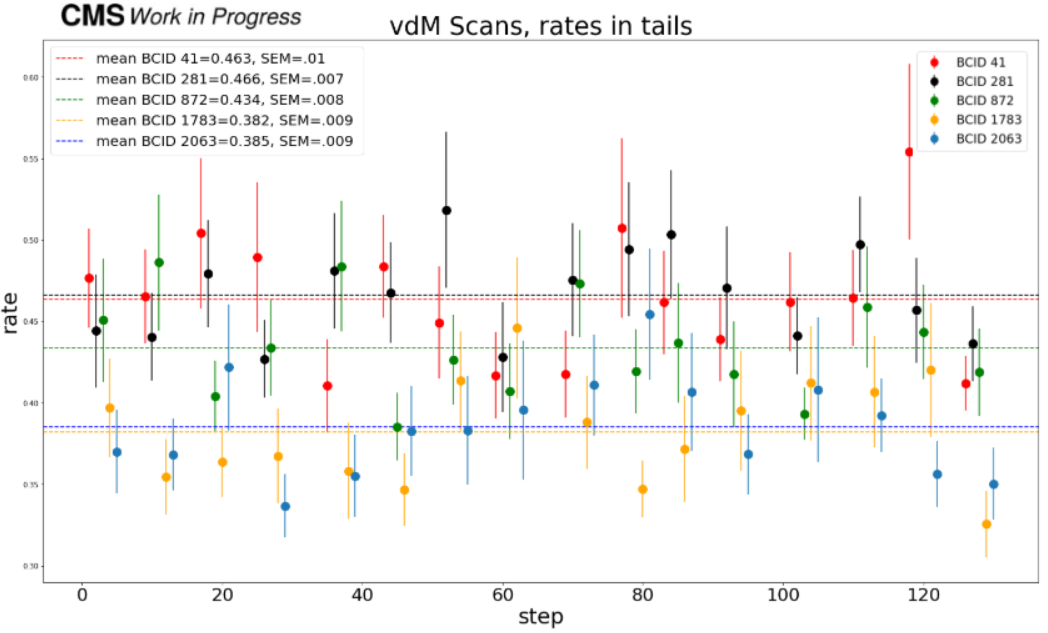
\includegraphics[width=0.5\textwidth,height=0.30\textwidth]{Chapter4/scan_rates_PerBX.png}
    \caption[Background Per BCID (2017)]{Left: Example of the average rates in a vdM scan for a single BCID. The tail values used in the study are highlighted with red circles. Right: Tail values from the scans and the mean background values per BCID.}
    \label{fig:SS_rates}
\end{figure}


For the 2018 vdM program, two Super-Separation scans (SS1 and SS2) were conducted to estimate the background value and its corresponding statistical error (SEM). The mean and standard deviation are obtained from the distribution resulting from the Y-projection of the $<\text{PCC}>$ rates during the period. This is done for each of the five BCIDs (265, 865, 1780, 2190, and 3380) selected for data acquisition that year. The process is performed individually for each SS period. Since the background noise values are consistent across different BCIDs, the final background value is determined by first averaging the five BCIDs within each SS period and then averaging the final values from both Super-Separation periods.

An example of an SS period I for BCID 265 and the calculation of the background level is shown in Fig.~\ref{fig:bx_265}. The left plot displays $<\text{PCC}>$, which represents the average number of pixel clusters per event over a period of 1.32s (NB4). The lower regions of the plot correspond to a 5-minute time window during which the beams were separated by a distance of $6\sigma_{b}$. The right plot shows the Y-projection of this distribution during the SS period, from which the mean and error are obtained.


\begin{figure}[h]
    \centering
    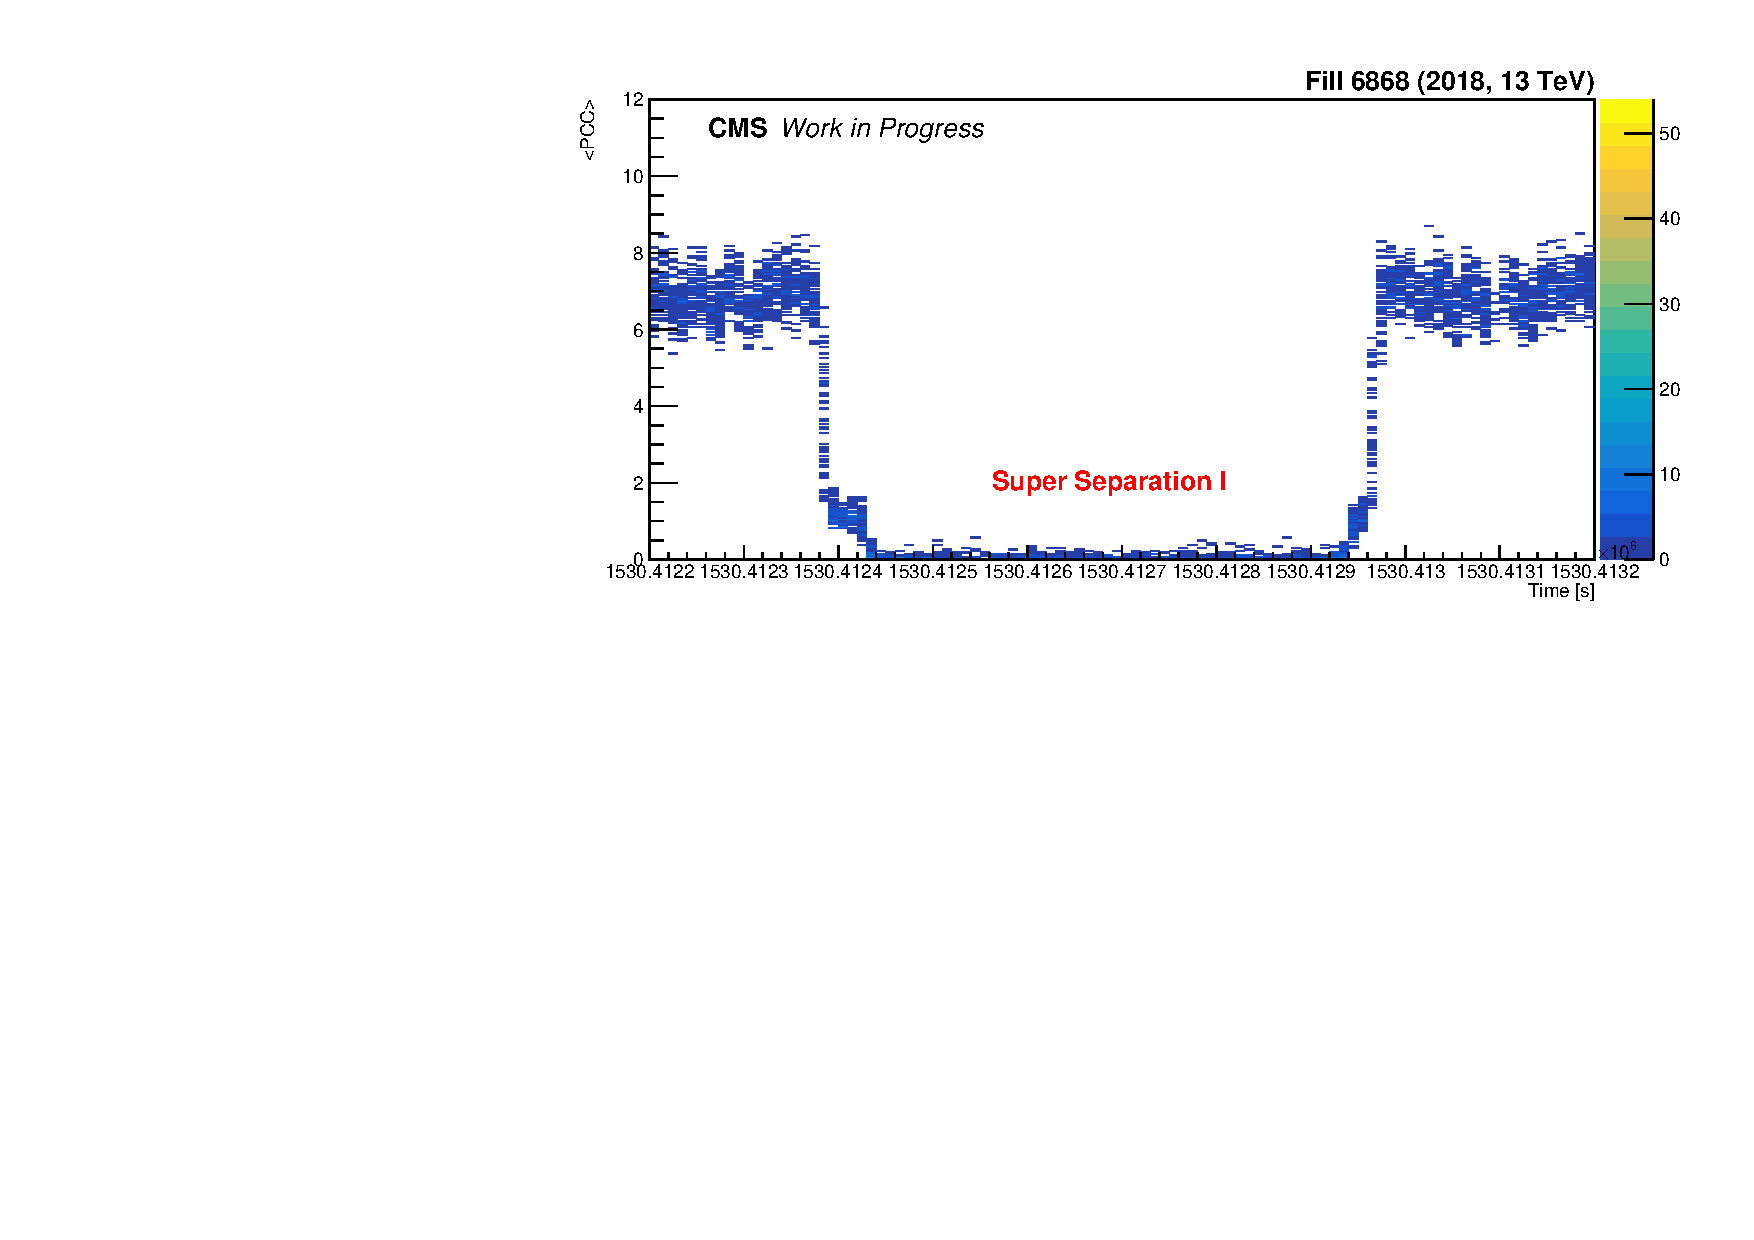
\includegraphics[width=0.44\textwidth,height=0.30\textwidth]{figures/performance_PCC/PCC_Rates_SS1.pdf}
    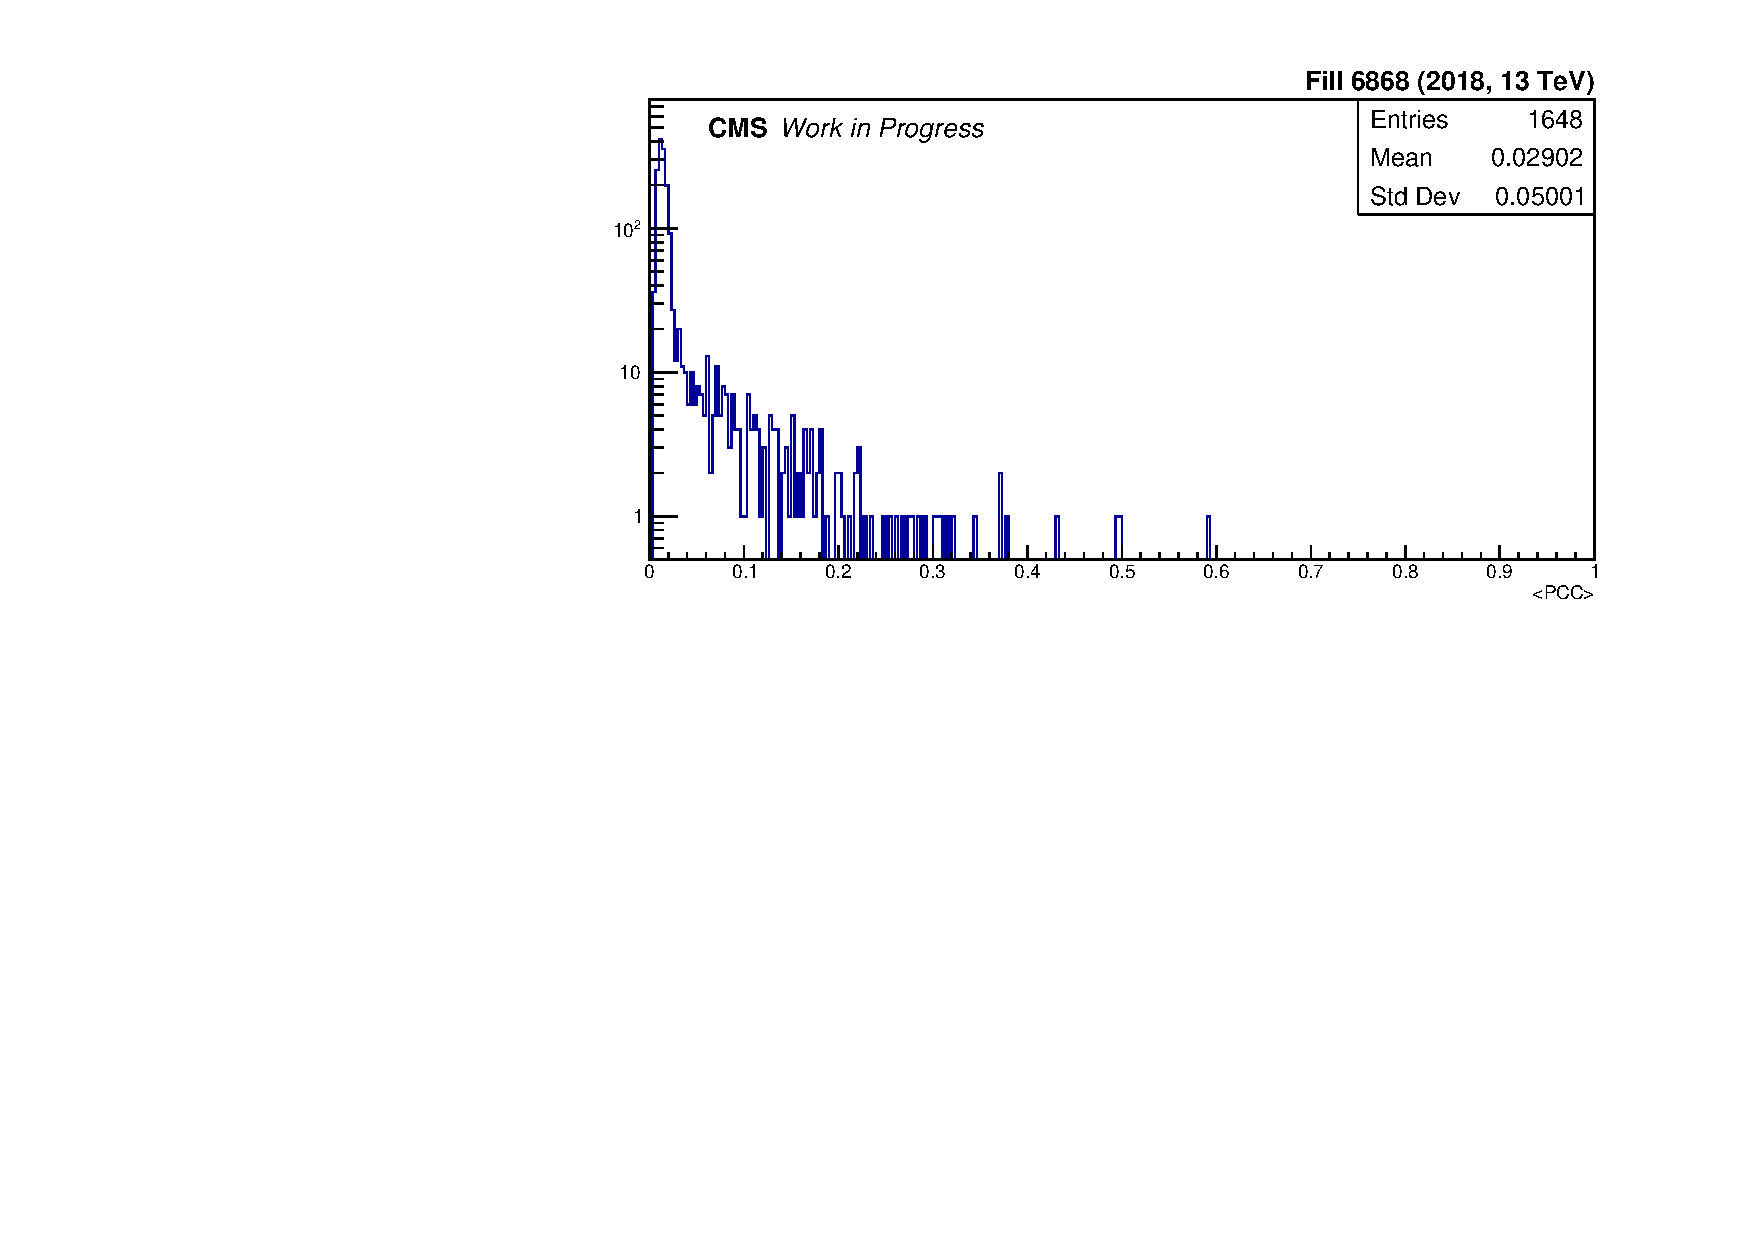
\includegraphics[width=0.54\textwidth,height=0.30\textwidth]{figures/performance_PCC/PCC_Projection_SS1.pdf}
    \caption[Background in BCID 265 during SS1 (2018)]{Left: PCC raw rates in Super Separation Period I in fill 6868 (2018) for BCID 265. 
    Right:PCC distribution corresponding to the Super Separation Period I for BCID 265.}
    \label{fig:bx_265}
\end{figure}

Finally, the background values for the five different BCIDs in 2017 and 2018 are shown in Table~\ref{tab:vdm_bkg}. In 2017, each BCID was corrected individually. For 2018, the final background correction applied to the PCC rate is $0.02757 \pm 0.01987$, obtained by averaging the BCIDs and SS periods.


\begin{table}[h]
    \caption{PCC background estimated for 2017 and 2018 vdM data.}
    \label{tab:vdm_bkg}
    \centering
    \begin{minipage}{0.45\textwidth}
        \centering
        \textbf{2017 Fill 6016} \\ 
        \begin{tabular}{cc}
            BCID & Bkg. \\ \hline
            41   & 0.463 \\
            281  & 0.466 \\
            872  & 0.434 \\
            1783 & 0.382 \\
            2063 & 0.385 \\
        \end{tabular}
    \end{minipage}
    %\hfill
     \hspace{1mm}
    \begin{minipage}{0.45\textwidth}
        \centering
        \textbf{2018 Fill 6868} \\ 
        \begin{tabular}{ccc}
            BCID  & Bkg. (SS1) & Bkg. (SS2) \\ \hline
            265   & 0.02902    & 0.02743    \\
            865   & 0.02572    & 0.02810    \\
            1780  & 0.02862    & 0.02860    \\
            2192  & 0.02729    & 0.02323    \\
            3380  & 0.02882    & 0.02896    \\
        \end{tabular}
    \end{minipage}
\end{table}







\section{Beam Corrections}
\label{bbcorrections}
%https://cms.cern.ch/iCMS/analysisadmin/cadilines?line=LUM-22-001

There are several systematic effects that affect the measurement of beam overlap width and therefore the extraction of $\sigma_{vis}$ from the vdM scan procedure. These effects are measured and, where applicable, corrected as described below. A systematic uncertainty is assigned to the resulting measured cross section $\sigma_{vis}$, and the following corrections are applied in the vdM Framework:
 
\begin{enumerate}

\item \textbf{Ghost and Satellites correction}. This correction addresses spurious charges in the machine that affect bunch currents. Satellite charges refer to additional charges beyond the 2.5 ns RF window containing the colliding bunch. Ghost charges correspond to charges beyond the 25 ns time window of nominally filled bunch slots.

The Longitudinal Density Monitors (LDMs) \cite{ghost_charge} measure these charges, and their correction follows the procedure described in Ref. \cite{lumi_precise_2015_2016}. If left uncorrected, they would bias the bunch population measurement and affect the determination of $\sigma_{\mathrm{vis}}$.

The correction to $\sigma_{\mathrm{vis}}$ is 0.02$\pm$0.05\% in 2017 and 0.09$\pm$0.03\% in 2018. Systematic uncertainties of 0.06\% and 0.07\% are assigned for 2017 and 2018, respectively. These uncertainties, attributed to instrumental effects, are considered correlated across both years.


\item \textbf{Bunch Current correction}. The LHC beam intensities, defined as the number of protons per bunch, are estimated from the bunch currents measured by the Fast Bunch Current Transformers (FBCT). These devices can resolve the particle multiplicity of individual bunches, denoted as $N_{\mathrm{FBCT}}^j$ \cite{LHC_bunch_populations}. A precise measurement of the total beam current, obtained by summing the individual bunch currents, is provided by the Direct Current Current Transformers (DCCTs). The total current, denoted as $N_{\mathrm{DCCT}$, is normalized to match the measured values with a relative precision of 0.2\%. This precision is directly assigned as a systematic uncertainty \cite{DCCT_calibration_studies}.


\item \textbf{Beam Beam corrections}. The electromagnetic interaction between colliding proton bunches affects beam-separation scans in two ways:

\textbf{Beam-Beam Deflection}. This correction accounts for the deflection of proton bunches during collisions, which causes a coherent shift in the nominal orbit. The electrical repulsion between the beams increases their lateral separation. This deflection is calculated and added to the nominal separation.

\textbf{Dynamic Beta}. The dynamic $\beta^{}$ effect, also known as the incoherent effect, accounts for changes in proton density distributions within the bunches due to single-particle interactions. These interactions alter the transverse bunch profiles during separation steps, which can be described as an effective change in the $\beta^{}$ value.

The corrections are calculated and applied individually for each bunch in each vdM scan. The average beam-beam interaction correction to $\sigma_{\mathrm{vis}}$ is 0.36\% for both years. The total uncertainties are 0.29\% in 2017 and 0.30\% in 2018, and they are considered fully correlated between the two years.


\item \textbf{Orbit drift correction}. This correction accounts for potential LHC orbit movements, including stochastic jumps and jitters (random changes in beam positions) during vdM scans. Time-dependent variations in transverse beam positions, even with fixed machine parameters, can alter beam separation. These changes are measured using beam position monitor (BPM) systems. The correction consists of two independent components:

\textbf{Linear Orbit drift}. This correction is divided into two components: Orbit Drift Separation (ODS), which accounts for orbit drift in the scanning direction and affects only beam separation, and Orbit Drift Rate (ODR), which corrects for orbit drift in the direction orthogonal to the scan, impacting only the luminometer rate. These effects result in a 0.13\% change in $\sigma_{\mathrm{vis}}$ in 2017 and 0.05\% in 2018.

\textbf{Residual orbit drift corrections}: accounts for beam position shifts not captured by linear orbit drift, length scale differences, or beam-beam deflection effects. A smooth function models the time-dependent drift, incorporating parameters to correct BPM scaling, beam-beam interaction magnitude and coordinate misalignments .The model is fitted using both scanning and non-scanning BPM data to ensure consistency. 


The final correction to the visible cross section including residual and linear orbit drift is 0.20\% in 2017 and 0.13\% in 2018, with uncertainties of 0.09\% and 0.19\%, respectively, which are correlated across years.


\item \textbf{Length Scale}. During beam separation scans, the beam positions are controlled by LHC dipole magnets, with separation determined by the magnet currents. To calibrate the absolute scale of these "nominal" positions, dedicated length scale calibration scans are conducted. These scans use a combination of methods: the constant-separation length scale scans, which track the movement of the luminous region (LR) through the mean reconstructed vertex position to calibrate the average length scale of the two beams in the transverse directions, and the variable-separation scans, which determine the LR position at the head-on configuration and compare it to the nominal beam position to compute the length scale. This approach measures the length scale of each beam separately in each direction. 

The procedure follows the method described in Ref. \cite{lumi_precise_2015_2016}. The correction to the visible cross section due to the length scale is -0.87 $\pm$ 0.12\% in 2017 and -0.66 $\pm$ 0.14\% in 2018.


\item \textbf{Transverse factorization}.

As mentioned in Section~\ref{vdM method}, the vdM method assumes that the bunch proton density is factorizable into independent $x$ and $y$ components, which can introduce a bias in the estimation of the beam overlap area. To evaluate and correct for this bias, dedicated beam imaging scans are used. Simulated vdM scan pairs are generated using the fitted transverse bunch density profiles, and the resulting luminous area ($2\pi\Sigma_{x}\Sigma_{y}$) is compared to the true beam overlap integral to quantify the factorization bias. This procedure, repeated multiple times, also accounts for statistical fluctuations and potential mismodeling associated with the chosen vdM fit function. To validate the modeling of the tails, luminous region fits are also performed using the scan combinations applied in the 2D rate-fit analysis. The average difference between the correction derived from the on-axis-only fit and that from the combined fit is added in quadrature to the uncertainty, yielding final uncertainties of 0.33\% and 0.36\% for 2017 and 2018, respectively.

\end{enumerate}



%https://indico.cern.ch/event/1244981/contributions/5230942/attachments/2581191/4452030/POG_pres.pdf
%\item Residual beam positions. To investigate additional deviations of the beams, a fit model is created by combining the nominal beam positions, the orbit drift correction, and the beam-beam deflection. In order to accommodate the unknown response of the Beam Position Monitors (BPM) to the beam-beam deflection, the beam-beam deflection is scaled using a parameter that is allowed to freely vary \cite{lumi_precise_2015_2016}. Moreover, length scale factors are also included as freely floating parameters. 

%In general, the residual deviations are less than 2 $\mum$. The primary source of uncertainty here is from the scale of the beam-beam deflection. Varying the scale parameter within the range of values found by the fit results in a change of $\sigma_{vis}$ of up to 1.0\%. This value is assigned as an uncertainty.\\

%\item Factorization bias. As we mentioned in section \ref{2022 vdM scan program} the vdM method assumes that the bunch proton density function is factorizable into dependent $x$ and $y$ distributions and this can lead to a biased estimate of the beam overlap area. For this, the special beam imaging scans are used. Wherein the measured vertex\footnote{A vertex is a hit recontruction that allow measure the location and the associated uncertainty, of all proton-proton interaction in each event \cite{vertex}} position distributions for $x$ and $y$ scans are fitted using aDouble Gaussian function \cite{BI_calibration,Measuring_luminosity}.

%\noindent For each fit result, the factorization bias is evaluated by comparing the luminous area ($2\pi\Sigma_{x}\Sigma_{y}$) with a simulation of a vdM scan pair that uses the fitted transverse proton bunch densities. This simulation is repeated several times to evaluate the impact of statistical fluctuations on the factorization bias. The  fit model results in a predicted factorization bias of about 0.7\% in $\sigma_{vis}$ . To account for potential additional contributions from higher order x-y correlations , twice the bias value is assigned as uncertainty.\\

%to estimate the rate at each scan step
%in the transverse bunch proton densities
 \\




\begin{comment}

\section{Fit Model  Selection}

After testing several mathematical fit models, the chosen model with the best fit quality and after applying all the corrections mentioned earlier, was a double Gaussian function:
%https://gitlab.cern.ch/bril/VdMFramework/-/blob/main/src/plotting/capsigma_over_time.py#L90
%\begin{equation}
%DG+Const= C+P \cdot \Biggl[ F \cdot \exp \Biggl( \frac{-(x-\bar{x})^{2}}{2 \sigma_{1}^{2} } \Biggr) + (1-F) \cdot \exp \Biggl( \frac{-(x-\bar{x})^{2}}{2 \sigma_{2}^{2} } \Biggr) \Biggr] 
%\end{equation}
%\begin{equation}
%f(x)= P \cdot \Biggl[ F \cdot \exp \Biggl( \frac{-(x-\bar{x})^{2}}{2(\frac{\Sigma\cdot R}{F \cdot R+1-F} )^{2} } \Biggr) + (1-F) \cdot \exp \Biggl( \frac{-(x-\bar{x})^{2}}{2 (\frac{\Sigma}{F \cdot R+1-F} )^{2} } \Biggr) \Biggr] 
%\end{equation}
%[5] + [2]*([3]*exp(-(x-[4])**2/(2*([0]*[1]/([3]*[1]+1-[3]))**2))
    %    + (1-[3])*exp(-(x-[4])**2/(2*([0]/([3]*[1]+1-[3]))**2)) )
%("#Sigma","#sigma_{1}/#sigma_{2}","peak","Frac","Mean","Const")
%[0] -> [0]*[1]/([3]*[1]+1-[3])
 %[1] -> [0]/([3]*[1]+1-[3])"""
 
 
\begin{equation} 
Poly4G(x)= A \Biggl[ 1+a_{2} \Biggl( \frac{-(x-\bar{x})}{\sigma} \Biggr)^{2} +a_{4} \Biggl( \frac{-(x-\bar{x})}{\sigma} \Biggr)^{4} \Biggr]\exp \Biggl[ -\frac{-(x-\bar{x})^{2}}{2\sigma^{2}}\Biggr]
\end{equation}
 
 
\begin{equation} 
Poly4G(x)= A \Biggl( 1+a_{2} \biggl( \frac{-(x-\bar{x})}{\sigma} \biggr)^{2} +a_{4} \biggl( \frac{-(x-\bar{x})}{\sigma} \biggr)^{4} \Biggr)\exp \Biggl( -\frac{-(x-\bar{x})^{2}}{2\sigma^{2}}\Biggr)
\end{equation}
 
\begin{itemize}
%\item $C$ is the constant value.
\item $P$ the $peak$ rate.
\item $F$ is the fraction of the peak rate attributed to the first Gaussian in the sum.
\item $x$ is the beam position.
\item $\bar{x}$ is the mean.
\item $\Sigma$ is the overlap between the beams.
\item $R$ is the ratio between the standard deviations of the  Gaussians (first over the second).
\end{itemize}

\end{comment}


\section{Visible cross section results}
\label{Visible cross section results}

In order to compute $\sigma_{\text{vis}}$, different combinations of Gaussian functions with adjustable parameters were tested to achieve the best fit. The selected model was the one that provided the highest fit quality, primarily determined by its convergence with the data points. This convergence is assessed using the covariance matrix, which quantifies the linear relationships between variables.

Another key criterion for evaluating fit quality is the chi-square ($\chi^2$) test, which determines whether the observed data follows a specified distribution (reference needed). A lower ($\chi^2$) value indicates a better fit.

After testing multiple mathematical models, the function that provided the best fit quality for both years, 2017 and 2018 data, was the "Poly4G" function, a combination of four Gaussian functions:


\begin{equation} 
Poly4G(x)= A \Biggl( 1+a_{2} \biggl( \frac{-(x-\bar{x})}{\sigma} \biggr)^{2} +a_{4} \biggl( \frac{-(x-\bar{x})}{\sigma} \biggr)^{4} \Biggr)\exp \Biggl( -\frac{-(x-\bar{x})^{2}}{2\sigma^{2}}\Biggr)
\end{equation}
 
\noindent where $A$ represents the peak rate, while $x$ corresponds to the beam position and $\bar{x}$ to the mean. The parameter $\sigma$ defines the overlap between the beams. Additionally, $a_{2}$ and $a_{4}$ are the coefficients associated with the Gaussian terms scaled by $x^2$ and $x^4$, respectively. 
 


%\begin{center}
\begin{figure}[h]
\centering
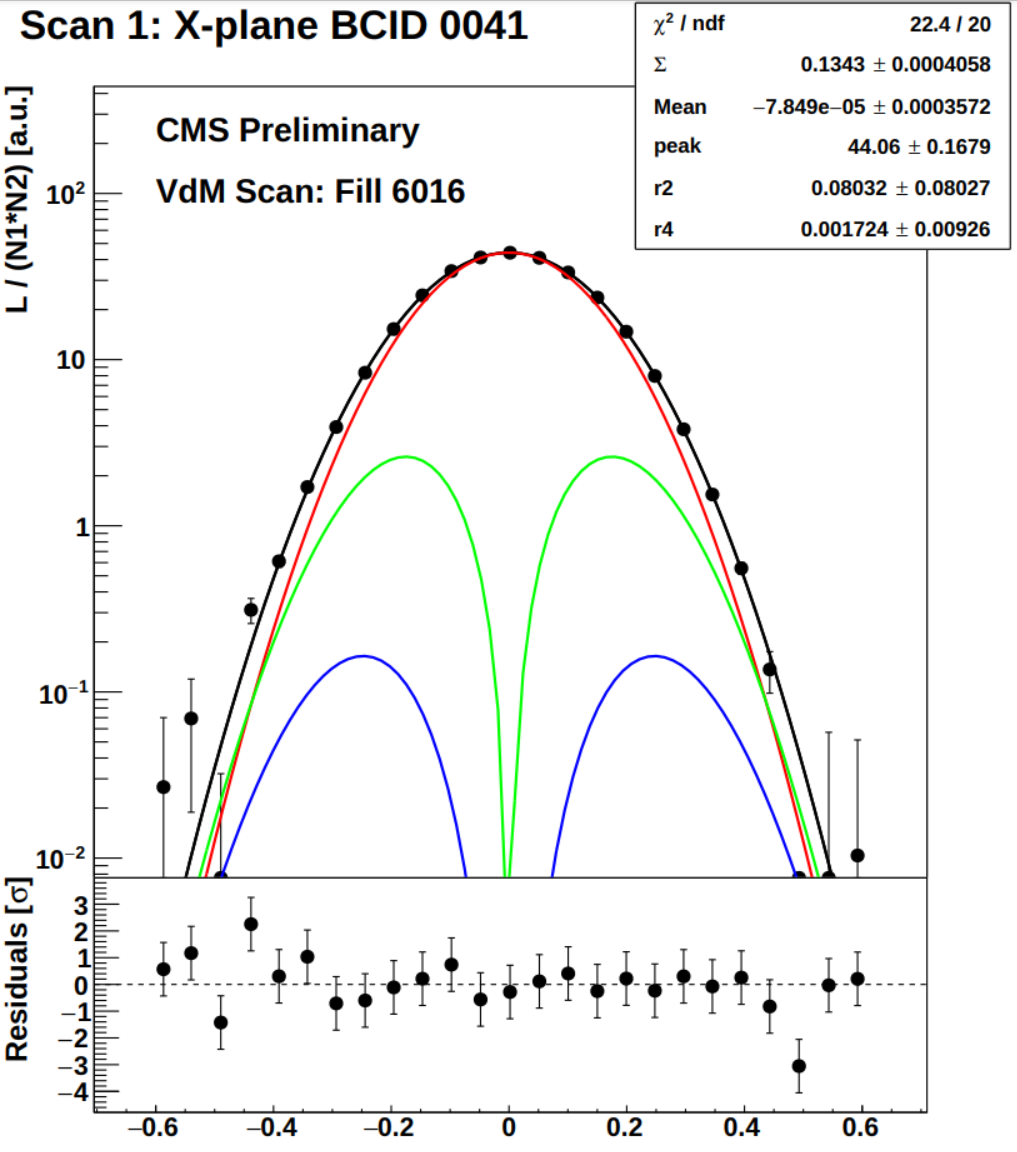
\includegraphics[width=.4\textwidth,height=0.4\textwidth]{Chapter4/2017_X_Scan_41.png}
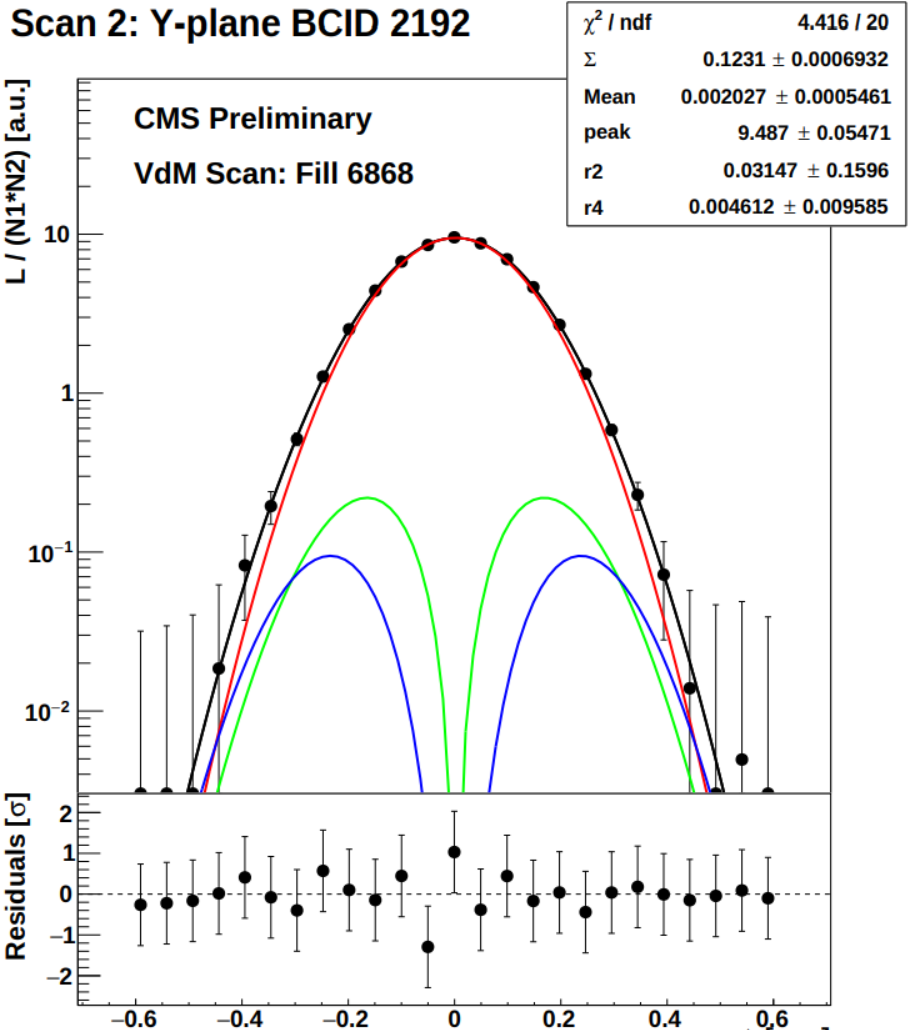
\includegraphics[width=.4\textwidth,height=0.4\textwidth]{Chapter4/2018_Y_Scan_2192.png}
\caption[Examples of Fits for vdM1: BCID 41 (2017) and BCID 2192 (2018)]{Normalized rates and the resulting fitted curves with  fit model as a function of the beam separation ($\Delta$) for the year 2017 BCID 41 in $x$ direction (left) and 2018 BCID 2192 in $y$ direction (right) both years for the vdM1 .}
\label{vdM1}
\end{figure}
%\end{center}


Finally, to compute $\sigma_{\text{vis}}$, the values of $\Sigma_{x,y}$ and $peak_{x,y}$ are extracted from each fit in the $x$ and $y$ directions. The visible cross section for each BCID (vdM and BI scans) is then determined using these fitted parameters, as illustrated in Fig. \ref{vdM1}. The final $peak$ value (P) is obtained by averaging the peaks from the $x$ and $y$ scans. For each bunch crossing, $\sigma_{\text{vis}}$ is computed using Eq. \ref{eq:sigVisX}. The error bars represent the uncertainty propagated from the fit, assigned as shown in Eq. \ref{sigma_err}, where $P = (R_{x}(0,0) + R_{y}(0,0))/2$.

\begin{equation}
 \sigma_{vis}= \pi \Sigma_{x} \Sigma_{y}P
 \end{equation}


\begin{equation}
\sigma_{vis\text{Err}}= 2 \pi \sqrt{ (\Sigma_{y} \cdot P \cdot \Sigma_{x\text{Err}})^{2} + (\Sigma_{x} \cdot P \cdot \Sigma_{y \text{Err}})^{2} + (\Sigma_{x} \Sigma_{y} P_{\text{Err}})^{2} }
\label{sigma_err}
\end{equation}

Figure \ref{sigmavis_perbcid} shows the value of $\sigma_{vis}$ per BCID along with its statistical error. The left panel corresponds to 2017 (4 vdM scans and 2 Img scans) for BCIDs 41, 281, 872, 1783, and 2063, while the right panel corresponds to 2018 (4 vdM scans and 3 Img scans) for BCIDs 265, 865, 1780, 2192, and 3380. A consistency within 0.1\% is observed among comparable channels for all luminometers, which we take as the uncertainty associated with the bunch-to-bunch variation of the derived visible cross sections.


\begin{center}
  \begin{figure}[h!]
    \centering
   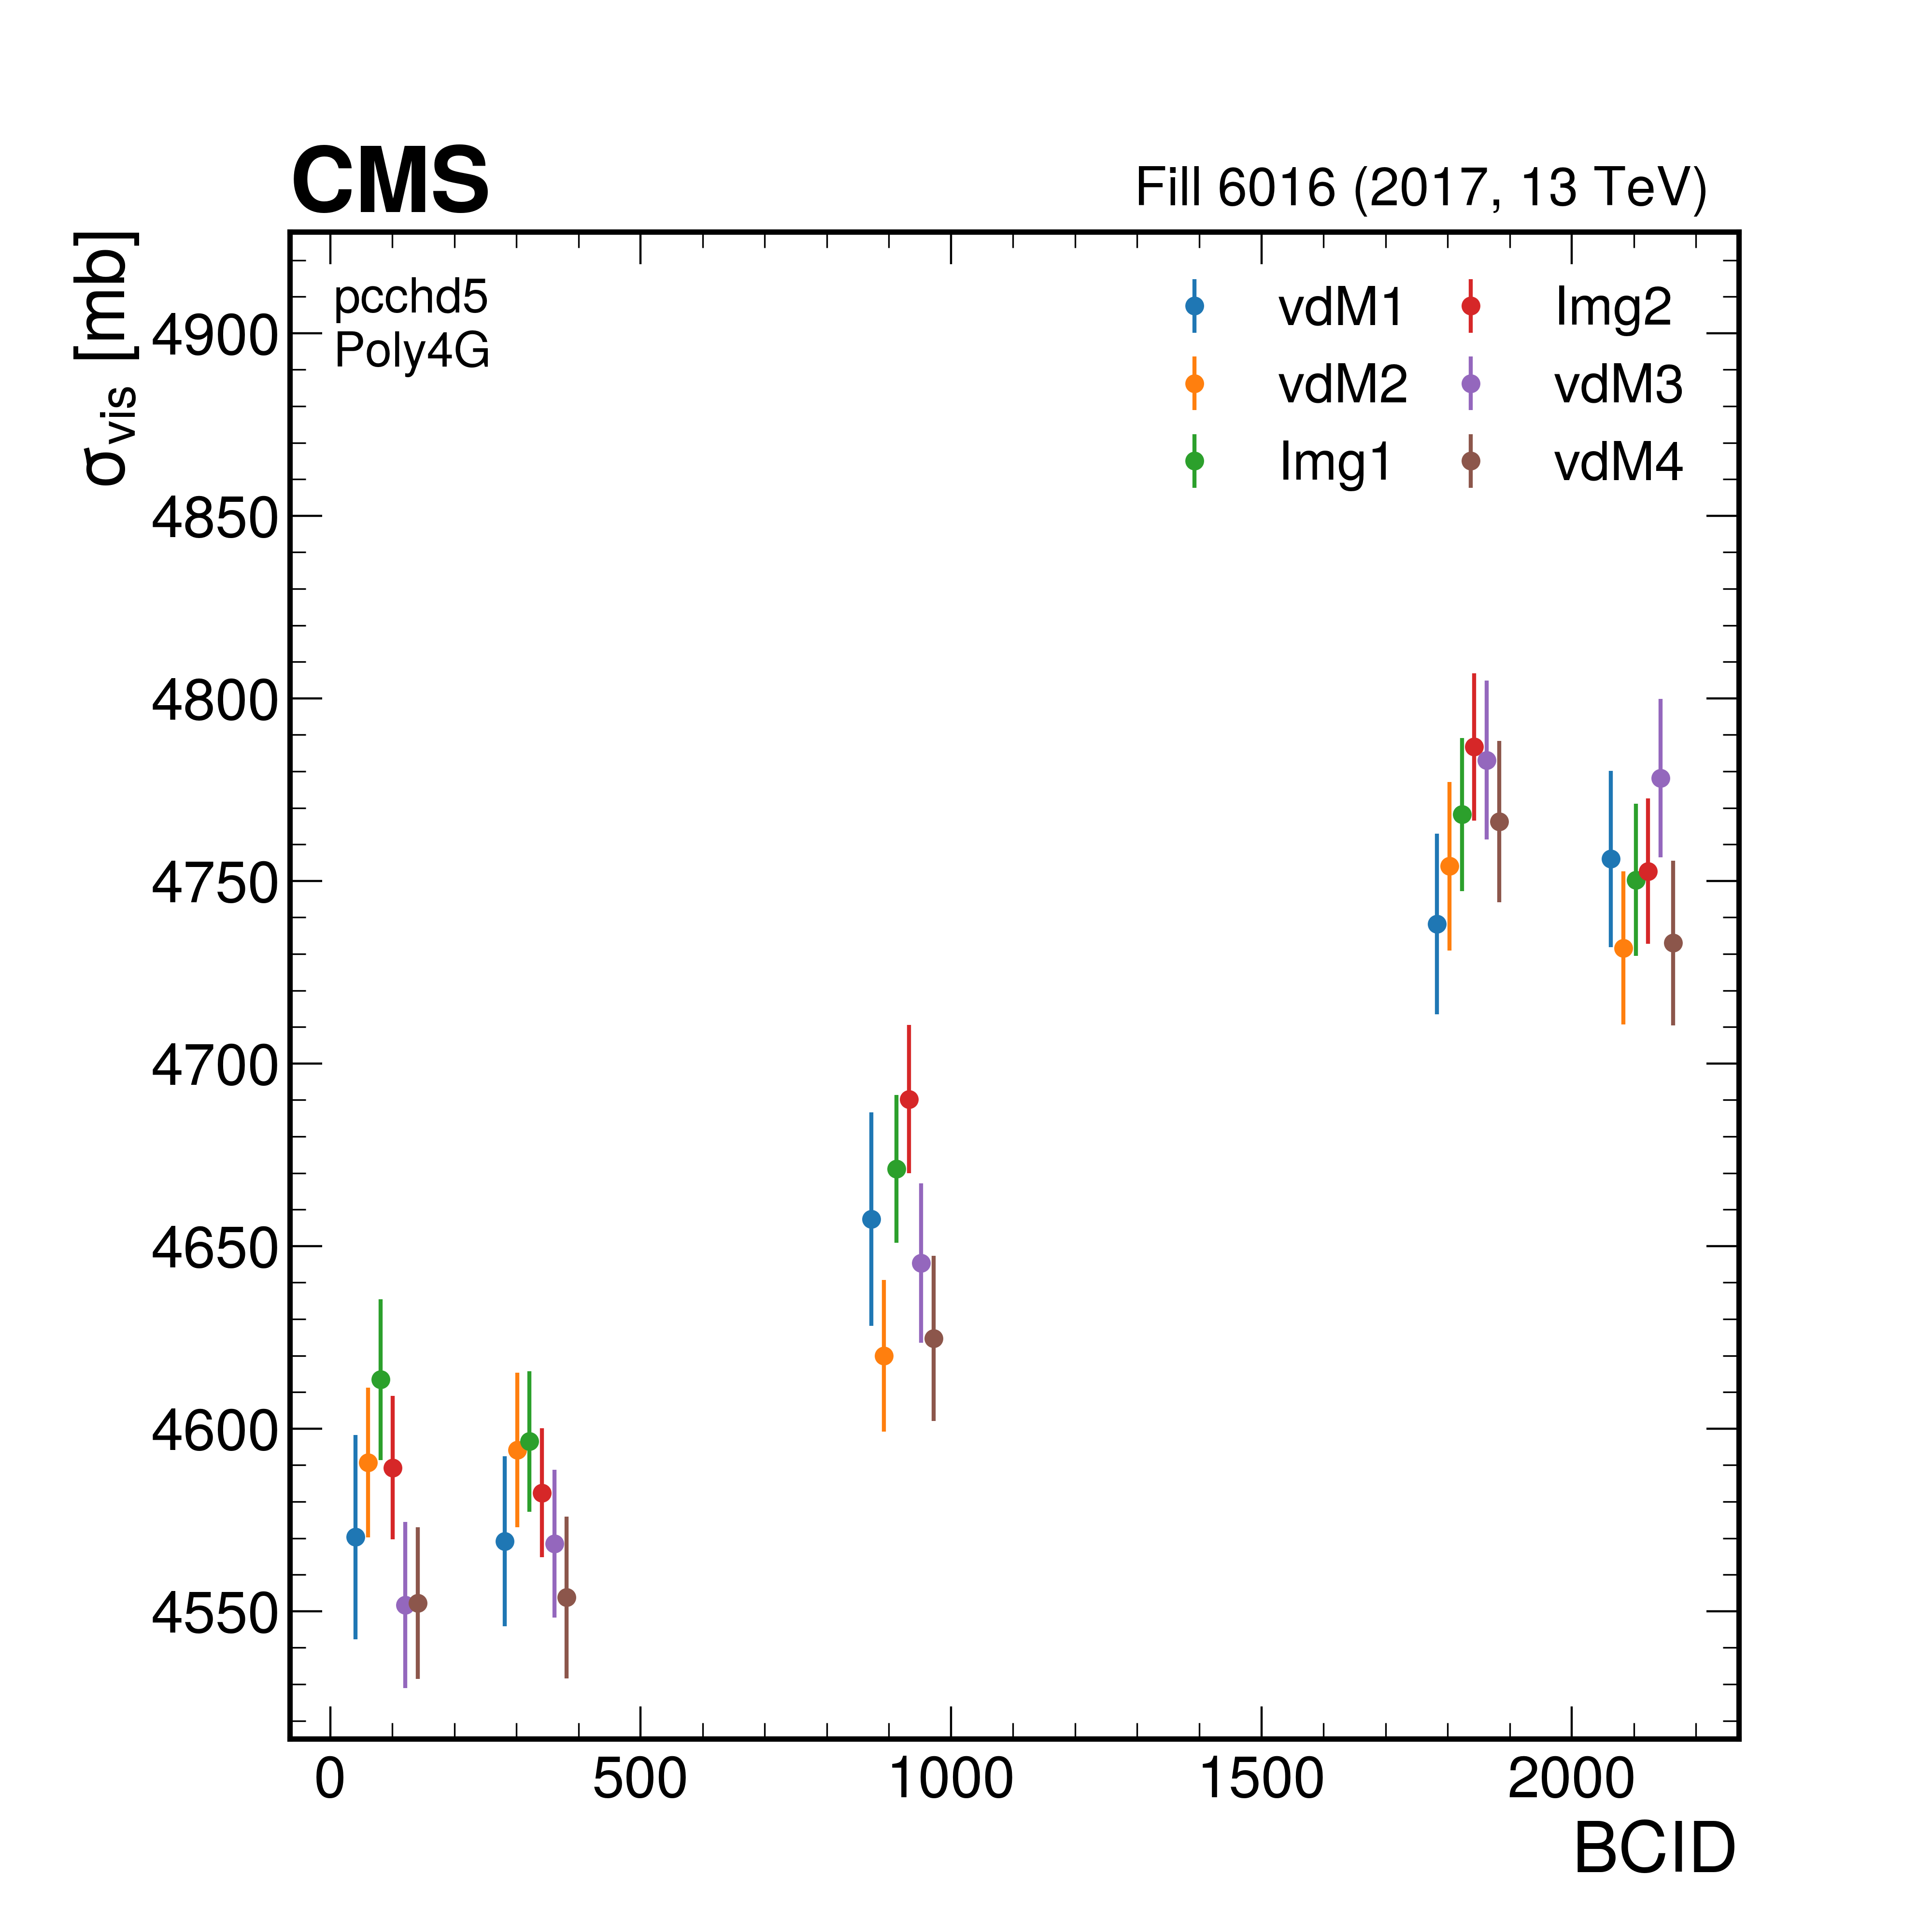
\includegraphics[width=.49\textwidth]{figures/vdMfitting/sigVis/Sigma_vis_6016_new_Per_BCID.png}
   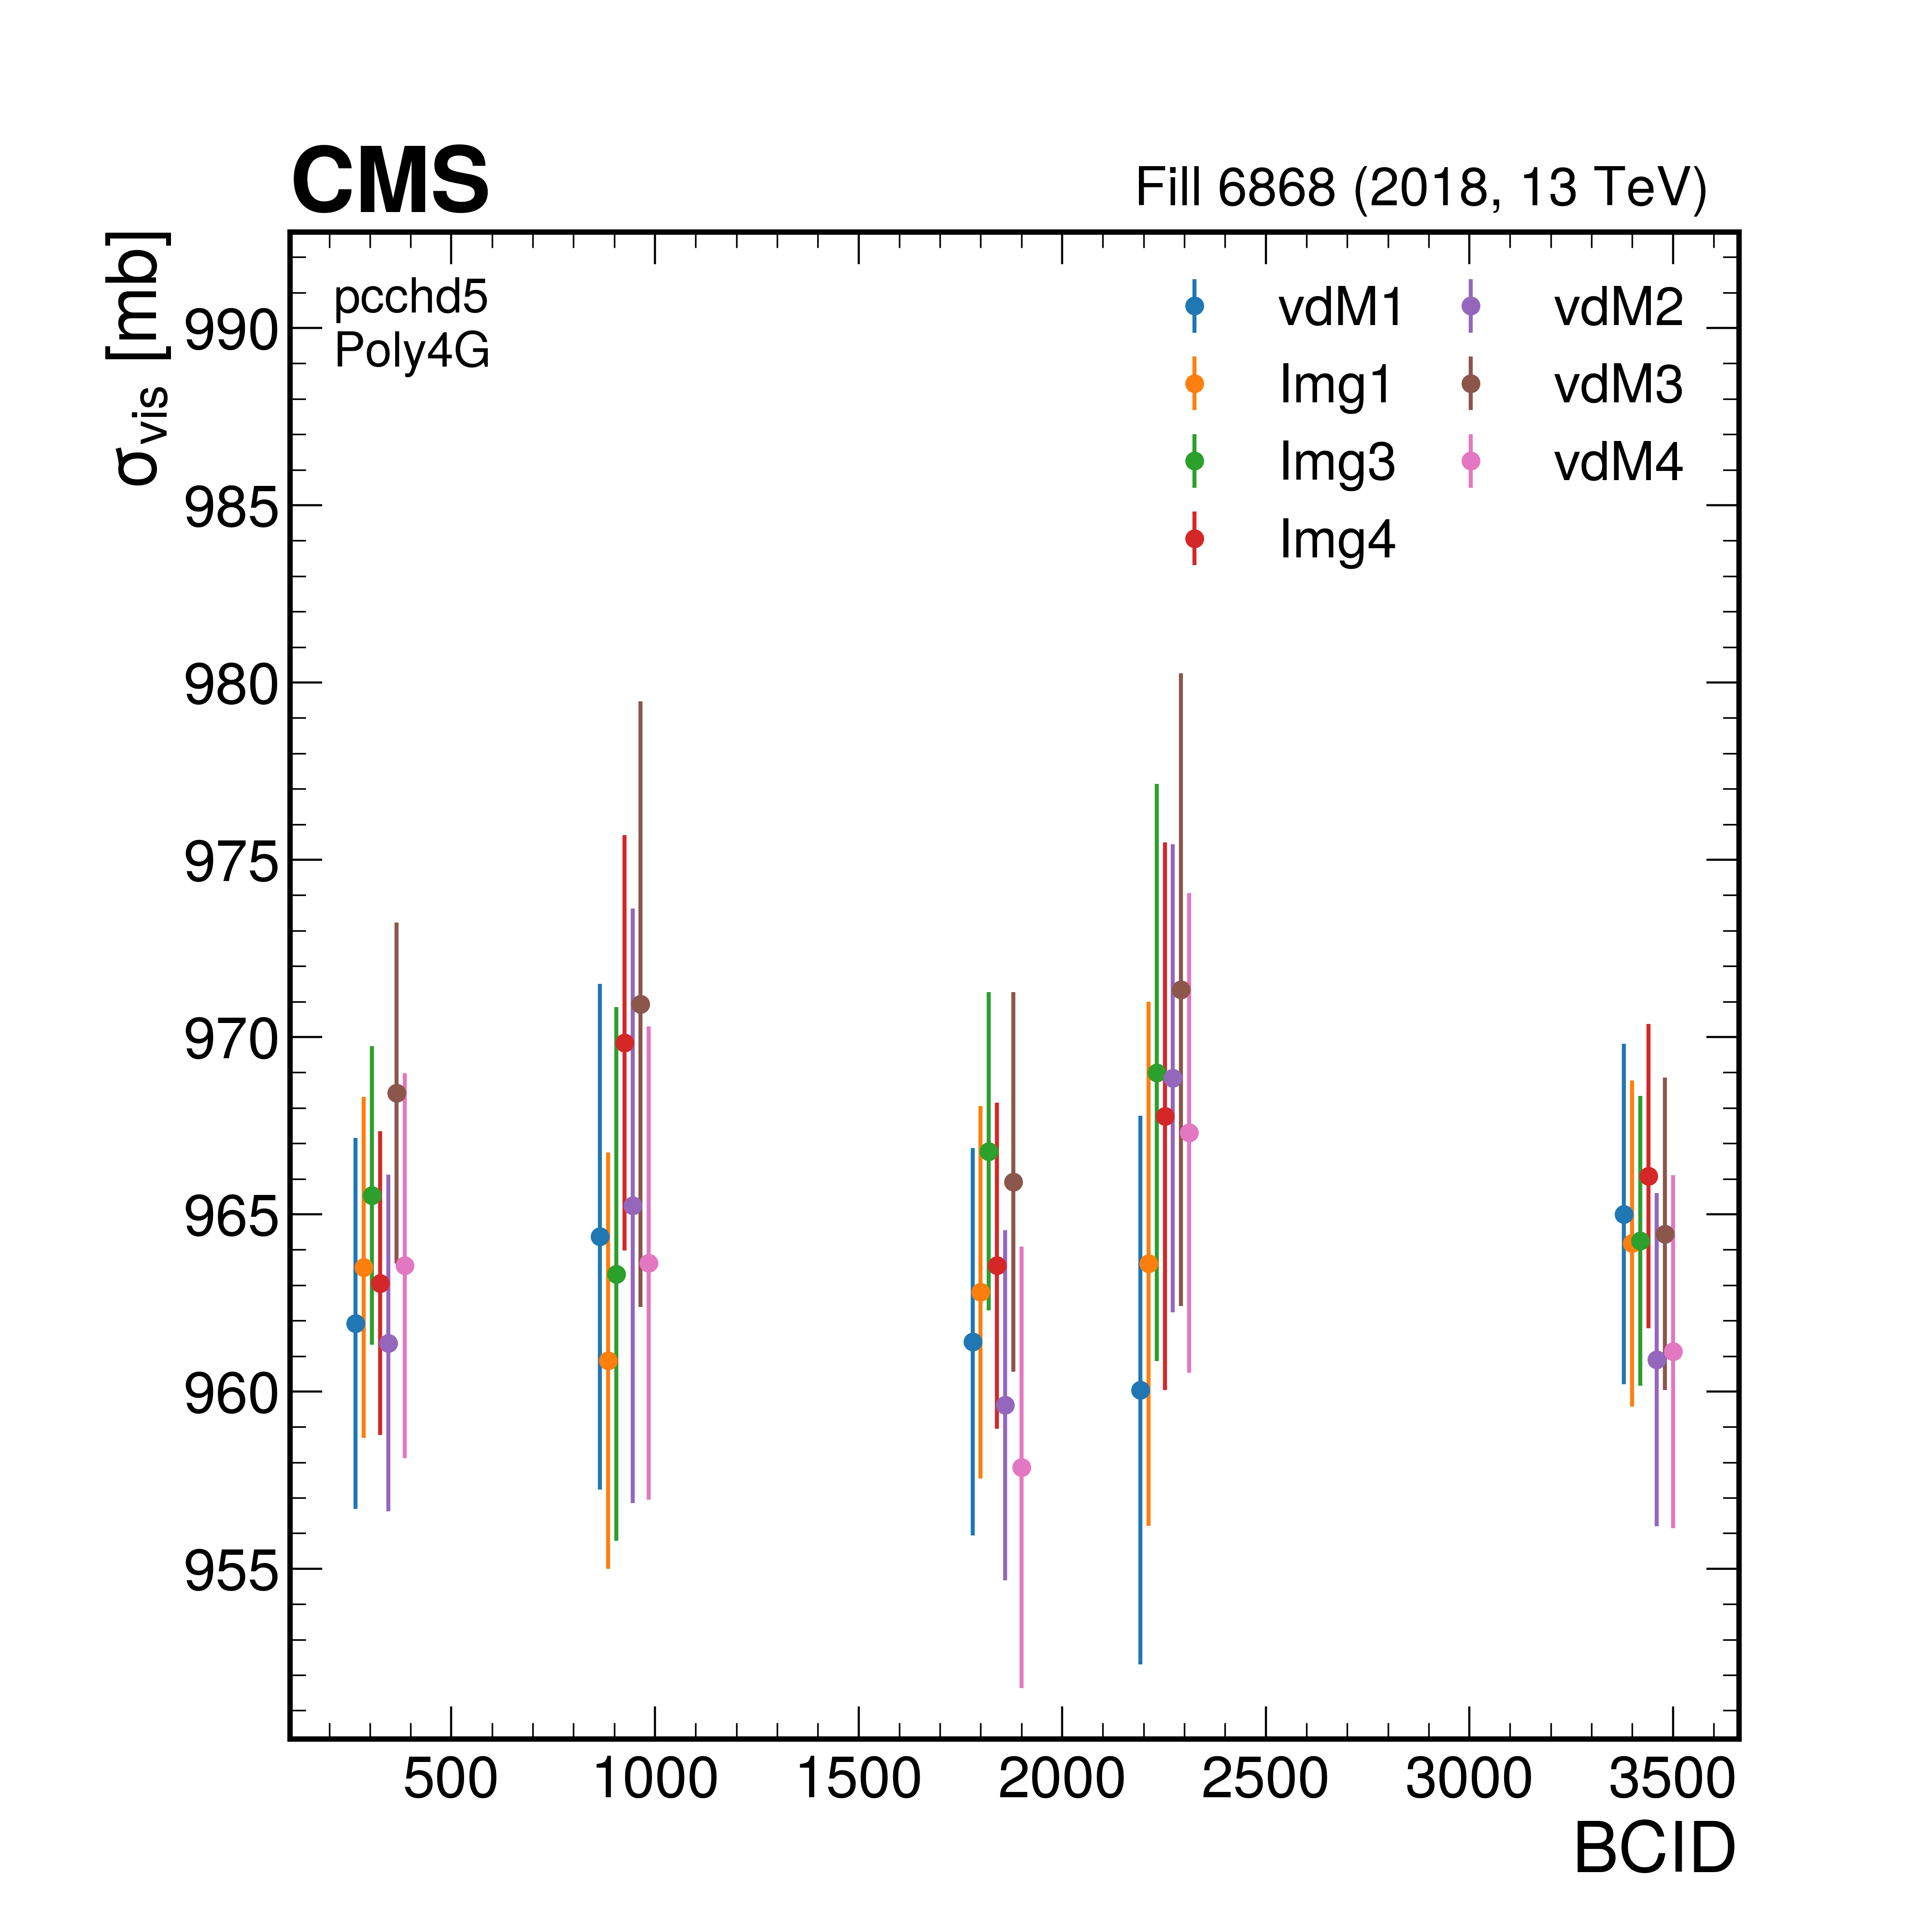
\includegraphics[width=.49\textwidth]{figures/vdMfitting/sigVis/Sigma_vis_6868_new_Per_BCID.png}
    \caption[$\sigma_{vis}$ per BCID for all scans]{ $\sigma_{vis}$ per BCID for all scans. In each scan, the BCIDs follow the same order: 41, 281, 872, 1783, and 2063 for 2017 (fill 6016), and 265, 865, 1780, 2192, and 3380 for 2018 (fill 6868).}
    \label{sigmavis_perbcid}
  \end{figure}
\end{center}

To obtain the final value of $\sigma_{\text{vis}}$, we first perform a weighted average using the five BCIDs for each scan. Then, we compute another weighted average across the results of these five scans. In both cases, we assume no correlation between the BCIDs and the scans. The weighted average per scan  and total error per scan  are calculated following Equations \ref{average} and \ref{error}, respectively, where the weight is defined as $ w_{i} = 1/\sigma_{\text{visErr}}^{2} $. 


\begin{eqnarray}
\sigma_{vis}^{Avg}=\Biggl(\displaystyle\sum_{i} w_{i}\sigma_{vis}^{i} \Biggr)\Biggl( \displaystyle\sum_{i} w_{i} \Biggr)^{-1}
\label{average}
\end{eqnarray}

\begin{eqnarray}
\sigma_{vis,Err}^{Avg}=\frac{1}{\sqrt{ \displaystyle\sum_{i} w_{i}}} 
\label{error}
\end{eqnarray}


The final result for $\sigma_{\text{vis}}$ is \textbf{4666.4 $\pm$ 14.7 mb} for 2017 and \textbf{964.9 $\pm$ 2.2 mb} for 2018. The final uncertainties are determined from the average standard deviation of the scan-to-scan results. These scan variations, along with those from other detectors, contribute to the final scan-to-scan variation uncertainty. Figure \ref{sigmavis_perscan} illustrates the per-scan values of the measured $\sigma_{\text{vis}}$ for PCC after all corrections. %A detailed summary of the visible cross-section values and their uncertainties for PCC in 2017 and 2018, for each applied correction, is presented in Table \ref{table:xsec3}, along with the percentage change in $\sigma_{\text{vis}}$.



%\begin{center}
\begin{figure}[h]
\centering
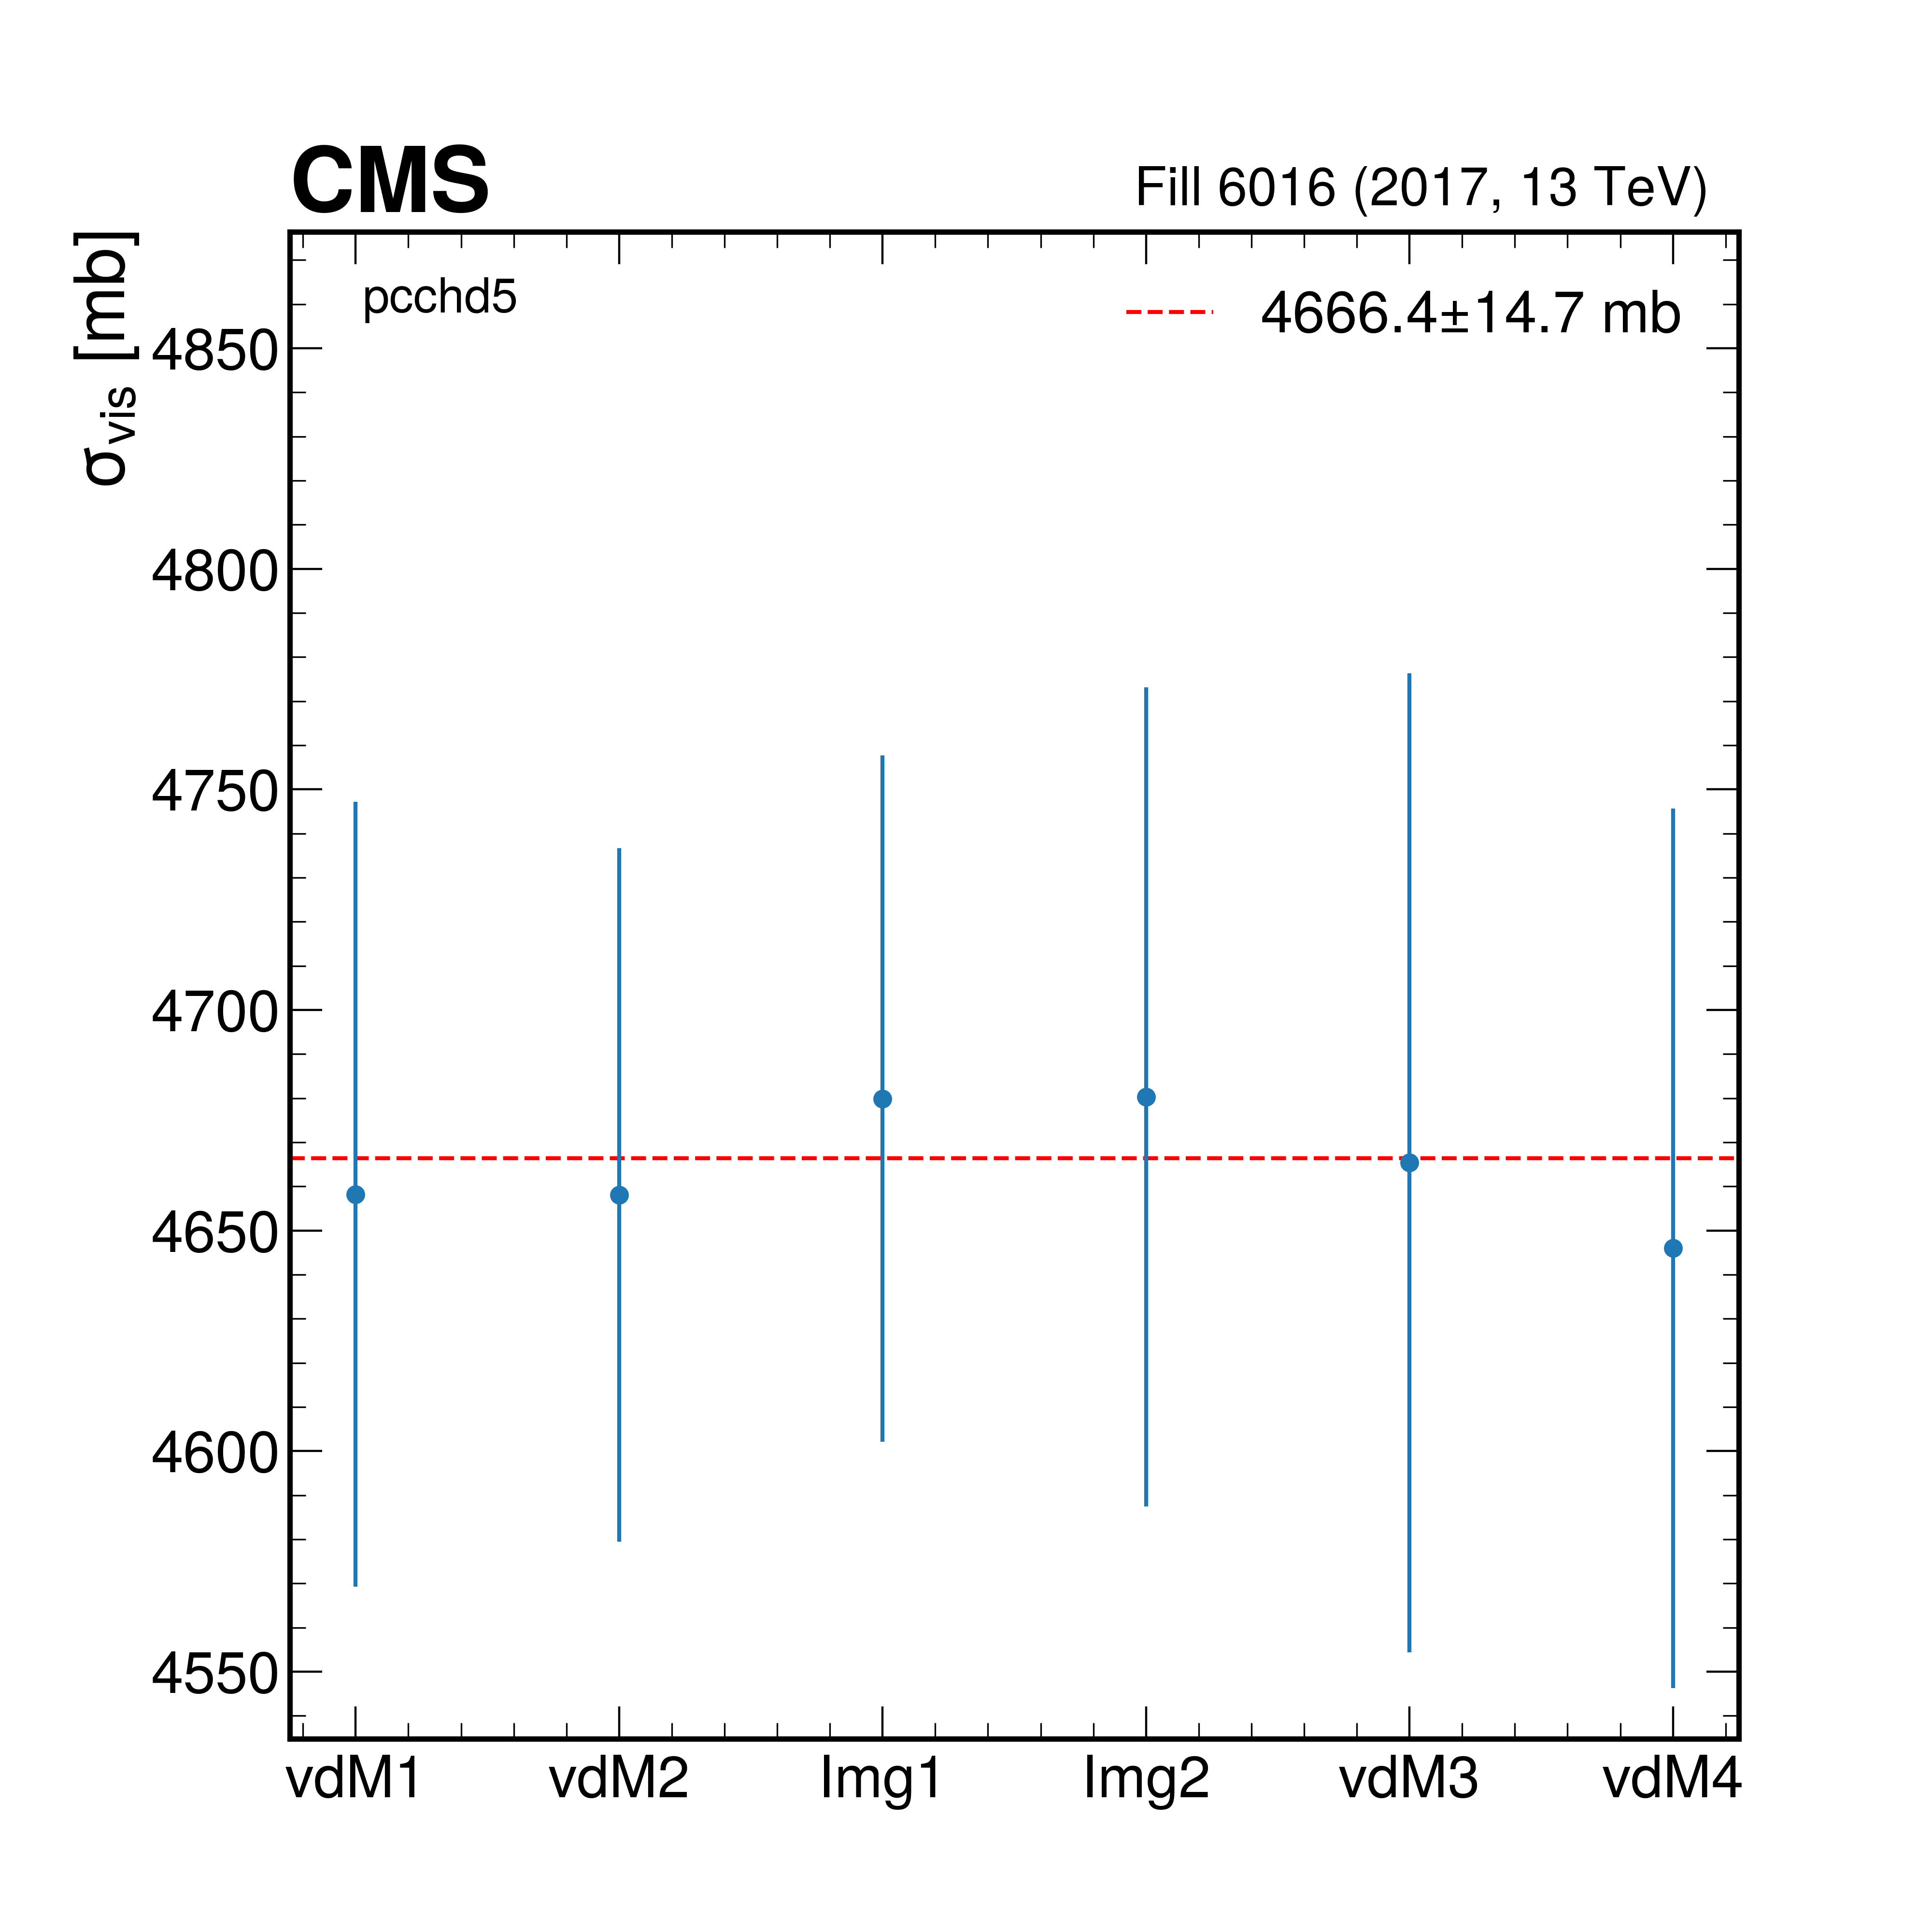
\includegraphics[width=.49\textwidth]{figures/vdMfitting/sigVis/Sigma_vis_6016_new.png}
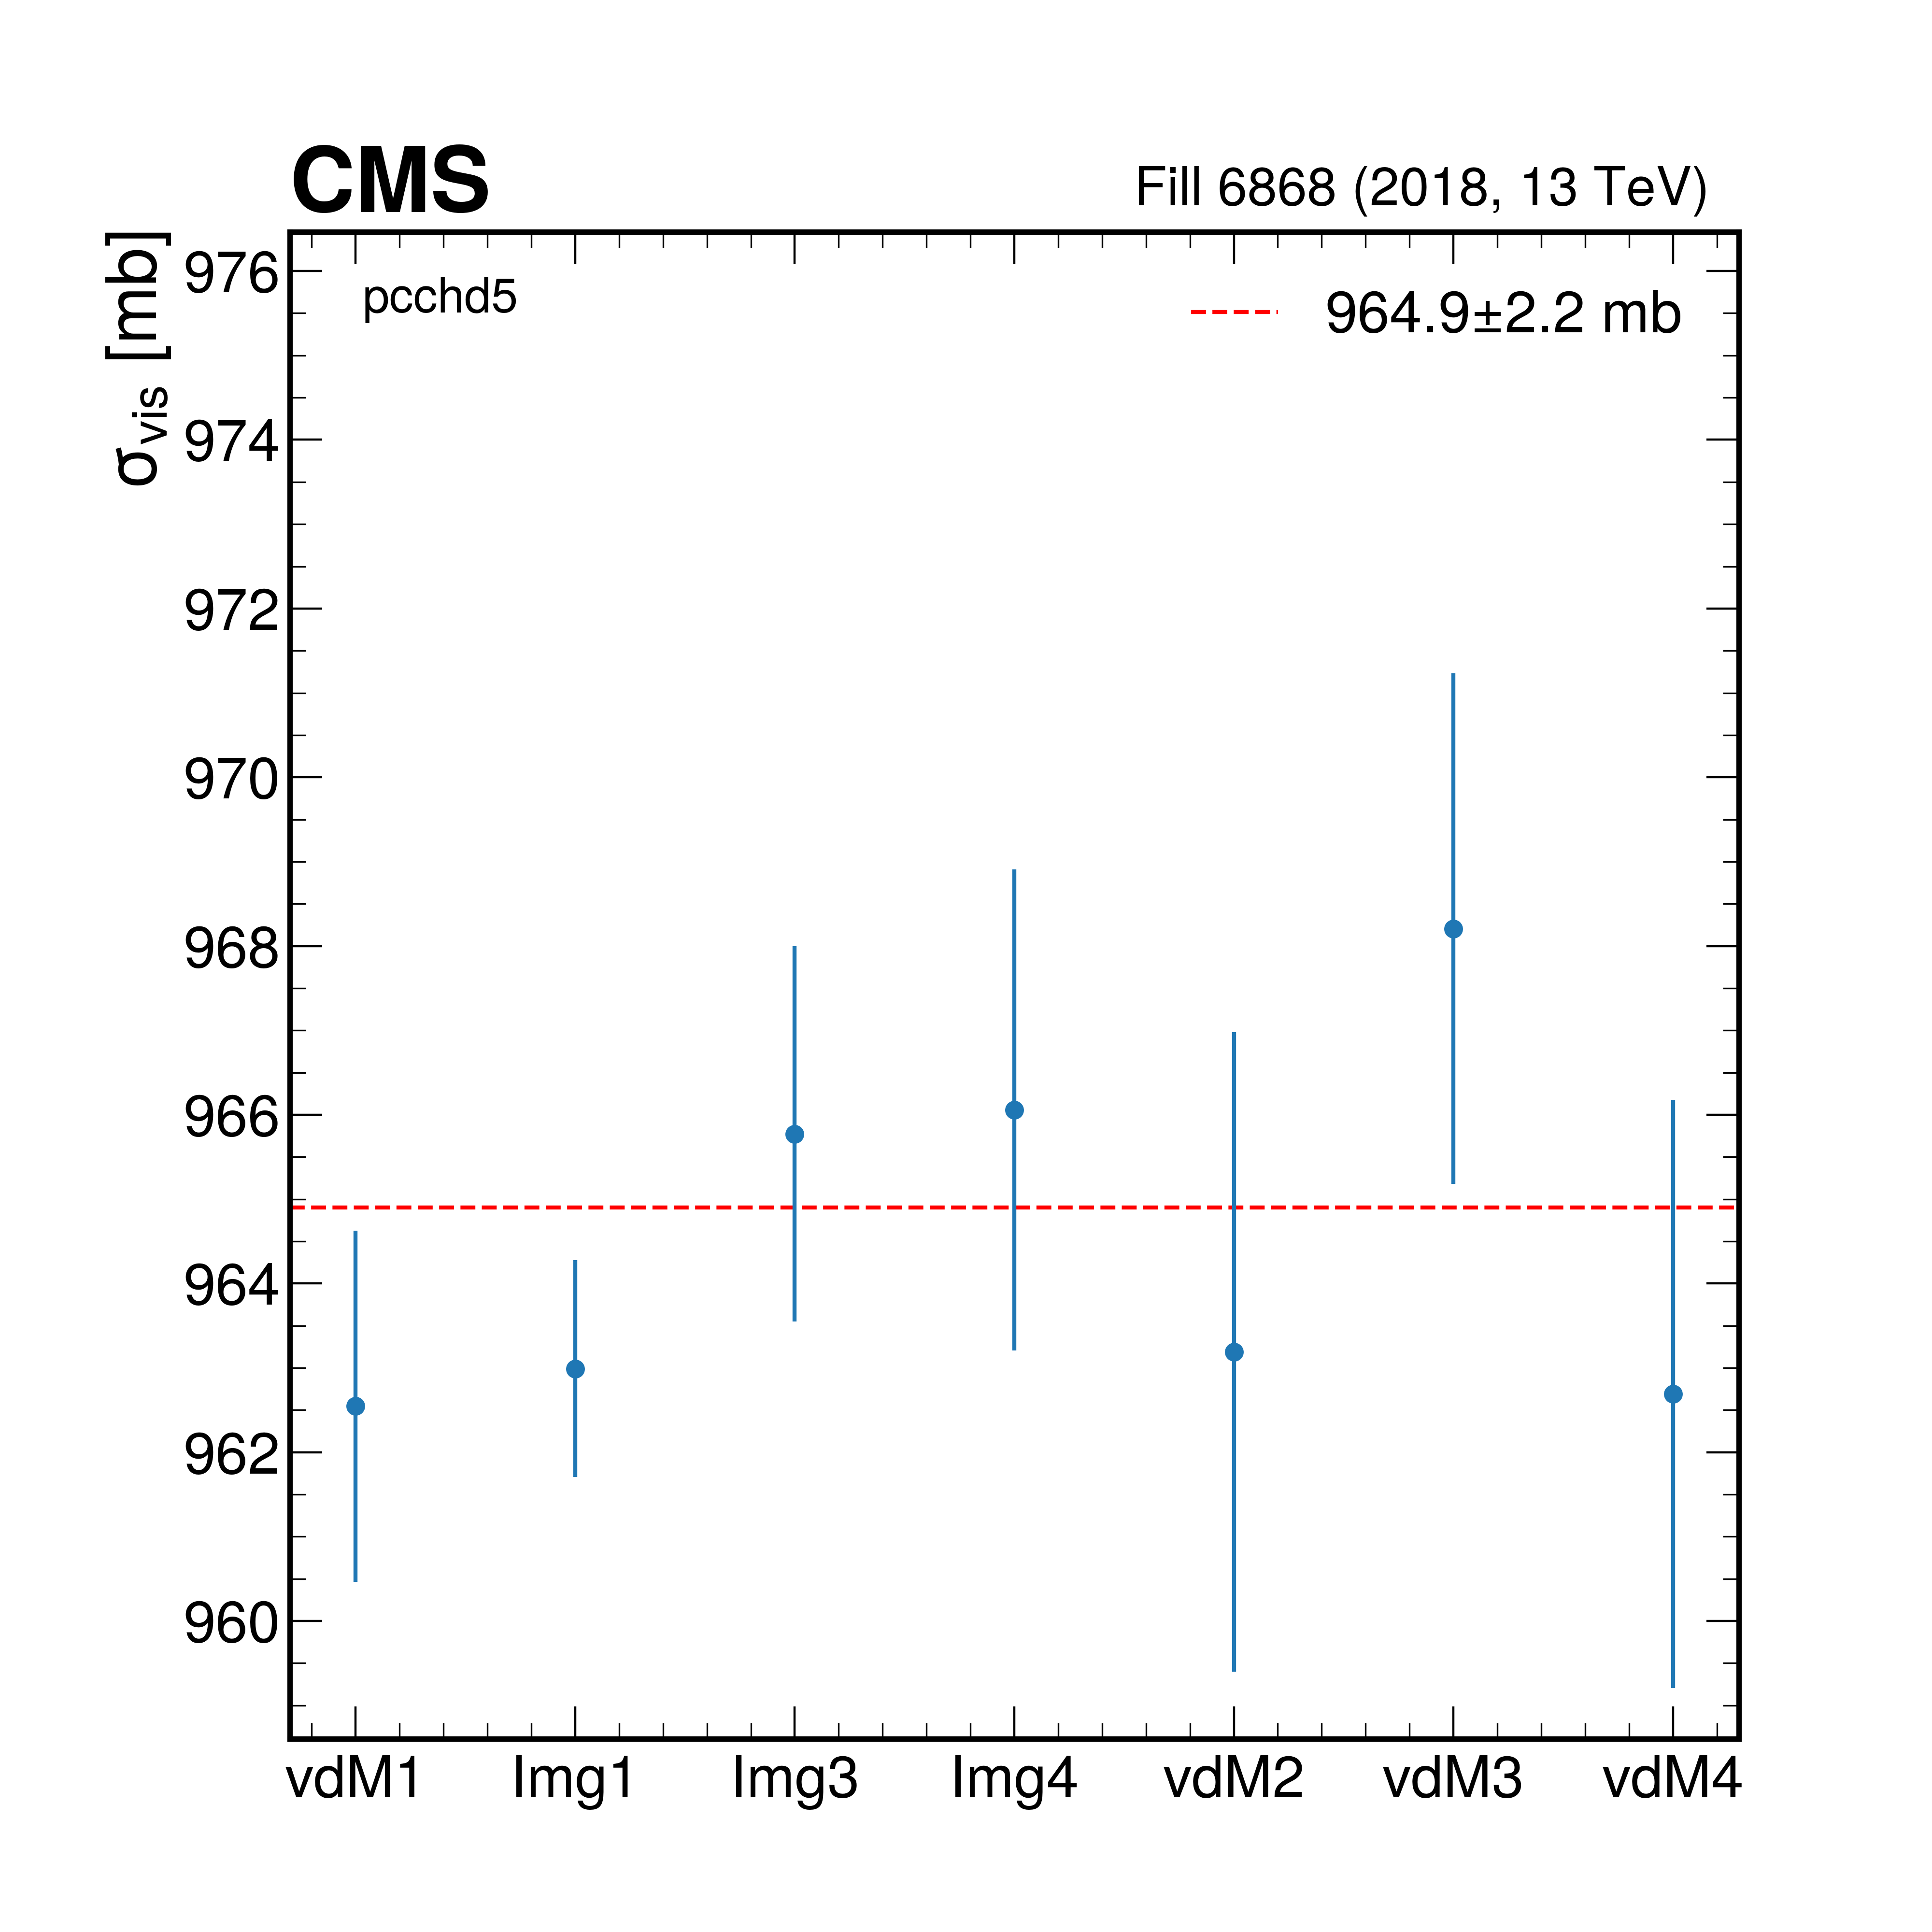
\includegraphics[width=.49\textwidth]{figures/vdMfitting/sigVis/Sigma_vis_6868_new.png}
\caption[$\sigma_{vis}$ average per scan and final result]{$\sigma_{vis}$ average per scan and final result}
\label{sigmavis_perscan}
\end{figure}
%\end{center}


\begin{comment}
\begin{table}[h]
\caption{ 
Summary of visible cross-section results for PCC in 2017 and 2018. Ghost and satellite corrections are applied in all rows. The corrections include BG for background correction, P2P for peak-to-peak correction, OD1 for orbit drift (OD) rate correction, OD2 for OD rate and separation correction, OD3 for OD2 plus residual orbit drift correction, BB for beam-beam correction, DB for dynamic $\beta^*$ correction, LS for length scale calibration, and XY for x-y correlations.}
\label{table:xsec3}
\begin{center}
\begin{tabular}{|c||c|c|}
\hline 
Correction & 2017 [mb] & 2018 [mb] \\ \hline 
 BG\_OD3\_BB\_DB\_LS\_P2P\_XY\_EC   & 4666.4$\pm$14.7 & 964.9$\pm$2.2 \\ 
 BG\_OD3\_BB\_DB\_LS\_P2P\_XY      & 4659.4$\pm$15.1 & 962.7$\pm$2.2 \\ 
 BG\_OD3\_BB\_DB\_LS\_P2P         & 4642.5$\pm$8.5 & 962.4$\pm$3.7 \\ 
 BG\_OD3\_BB\_DB\_LS             & 4641.4$\pm$9.6 & 962.3$\pm$3.7 \\ 
 BG\_OD2\_BB\_DB\_LS             & 4631.5$\pm$18.8 & 960.9$\pm$3.4 \\  BG\_OD2\_BB\_DB                & 4672.0$\pm$18.9 & 967.3$\pm$3.4 \\ 
 BG\_OD2\_BB                   & 4723.3$\pm$19.3 & 978.2$\pm$3.7 \\ 
 BG\_OD2                      & 4644.2$\pm$18.8 & 962.0$\pm$3.2 \\ 
 BG\_OD1                      & 4640.3$\pm$22.0 & 961.5$\pm$3.0 \\ 
 BG                          & 4638.0$\pm$20.5 & 961.4$\pm$4.0 \\ 
 noCorr                      & 5087.9$\pm$70.1 & 995.3$\pm$6.2 \\
\hline \hline
Emittance Change            & 0.15\% & 0.22\% \\ 
 Non-factorisation           & 0.36\% & 0.04\% \\ 
 Peak to Peak                & 0.02\% & 0.01\% \\ 
 Residual OD                 & 0.22\% & 0.14\% \\ 
 Length Scale                & -0.87\% & -0.66\% \\ 
 Dynamic Beta                & -1.09\% & -1.11\% \\ 
 Beam-Beam                   & 1.70\% & 1.68\% \\ 
 OD Rate                     & 0.08\% & 0.05\% \\ 
 OD Sep                      & 0.05\% & 0.01\% \\ 
 Background                  & -8.84\% & -3.41\% \\
\hline 
\end{tabular}
\end{center}
\end{table}
\end{comment}


Finally, Figure~\ref{fig:vdM_fit_sigVis_All} shows the scan-by-scan variations of the $\sigma_{\text{vis}}$ with all corrections for all detectors (PLT, PCC, HFET, and HFOC) and normalized to their average value taken over all scans to bring them onto the same scale. The average standard deviation of 0.26\% in 2017 and 0.27\% in 2018 is then taken into account as the final scan-to-scan uncertainty.


\begin{figure}[!h]
\centering
  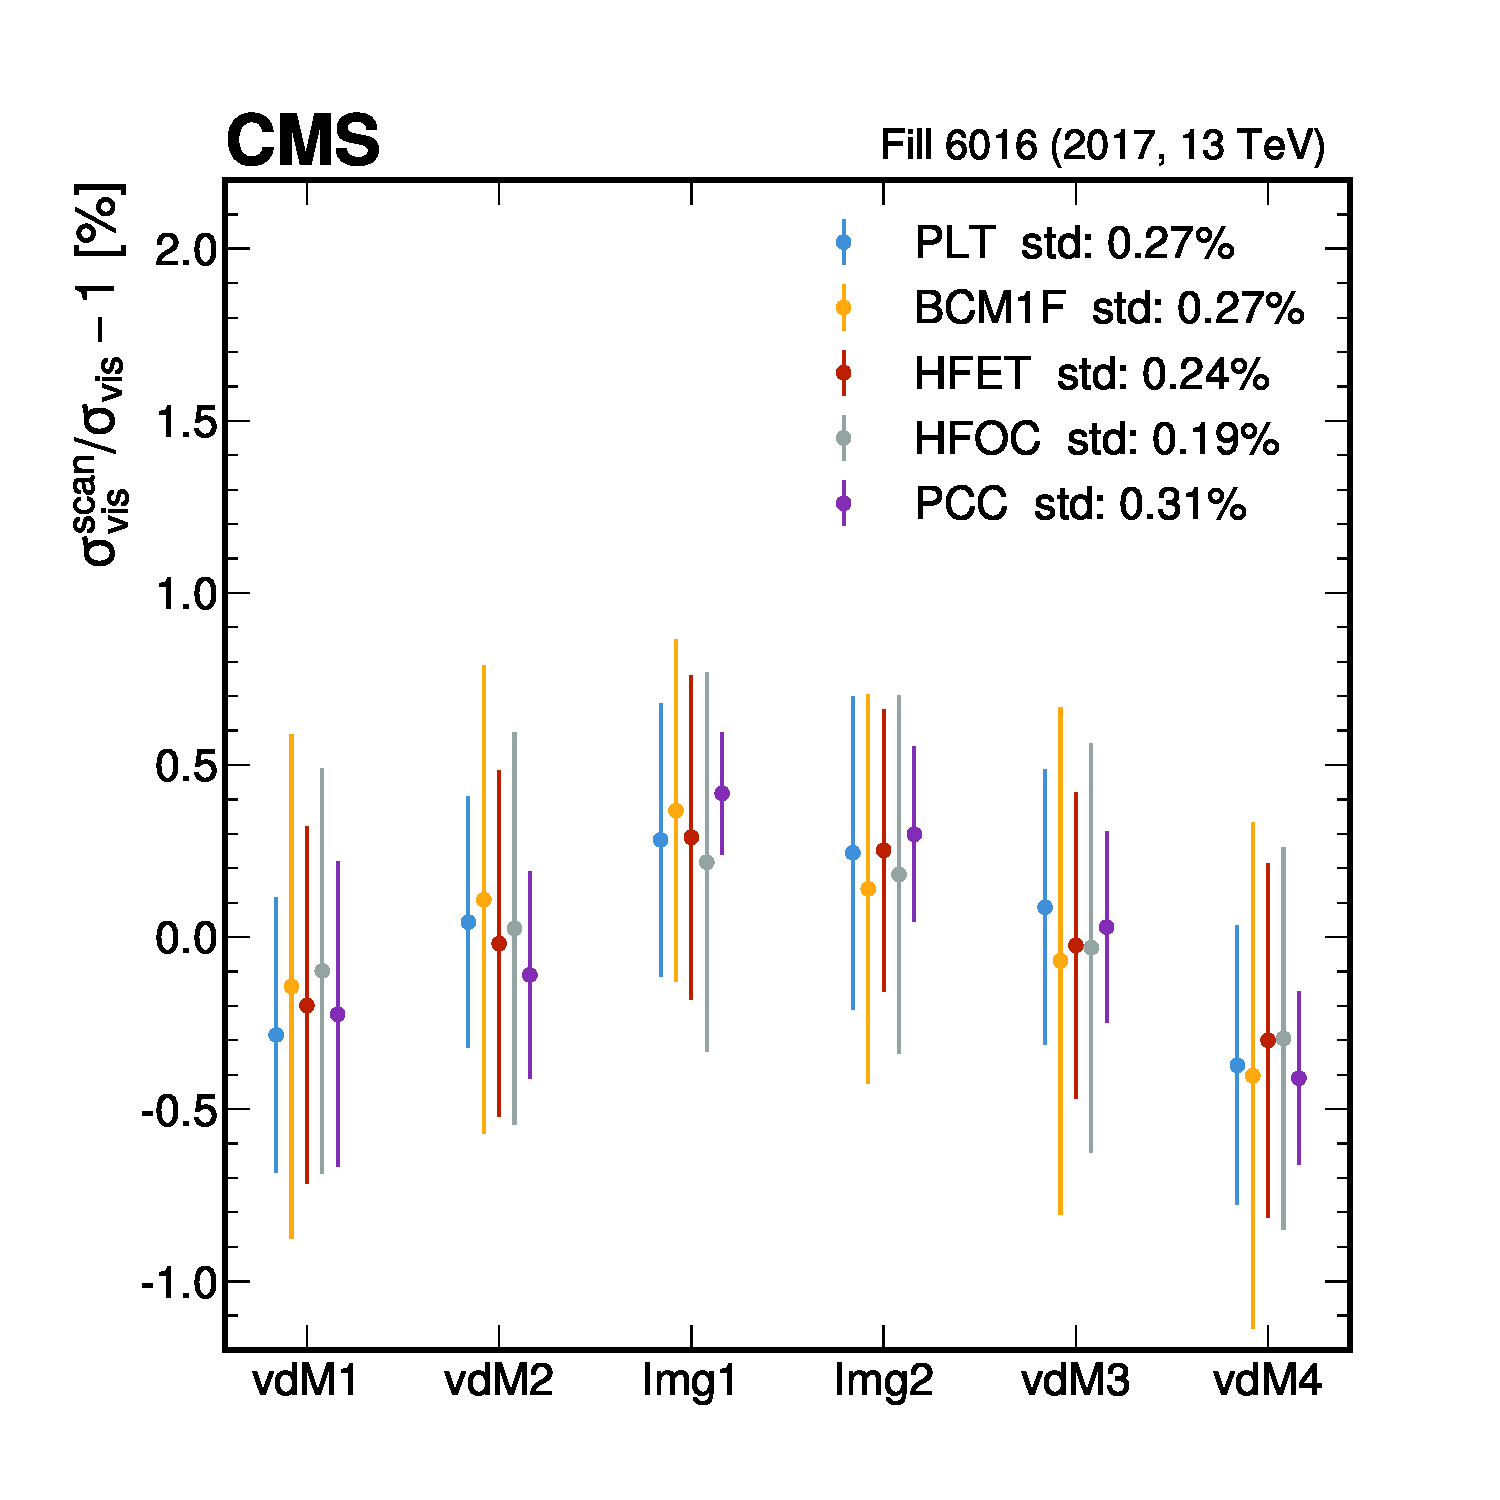
\includegraphics[width=0.49\textwidth]{figures/visible_cross_section_results/sigVisPerScanNormalized_fill6016_XY_EC.pdf}
  %\hspace{0.05\textwidth}
  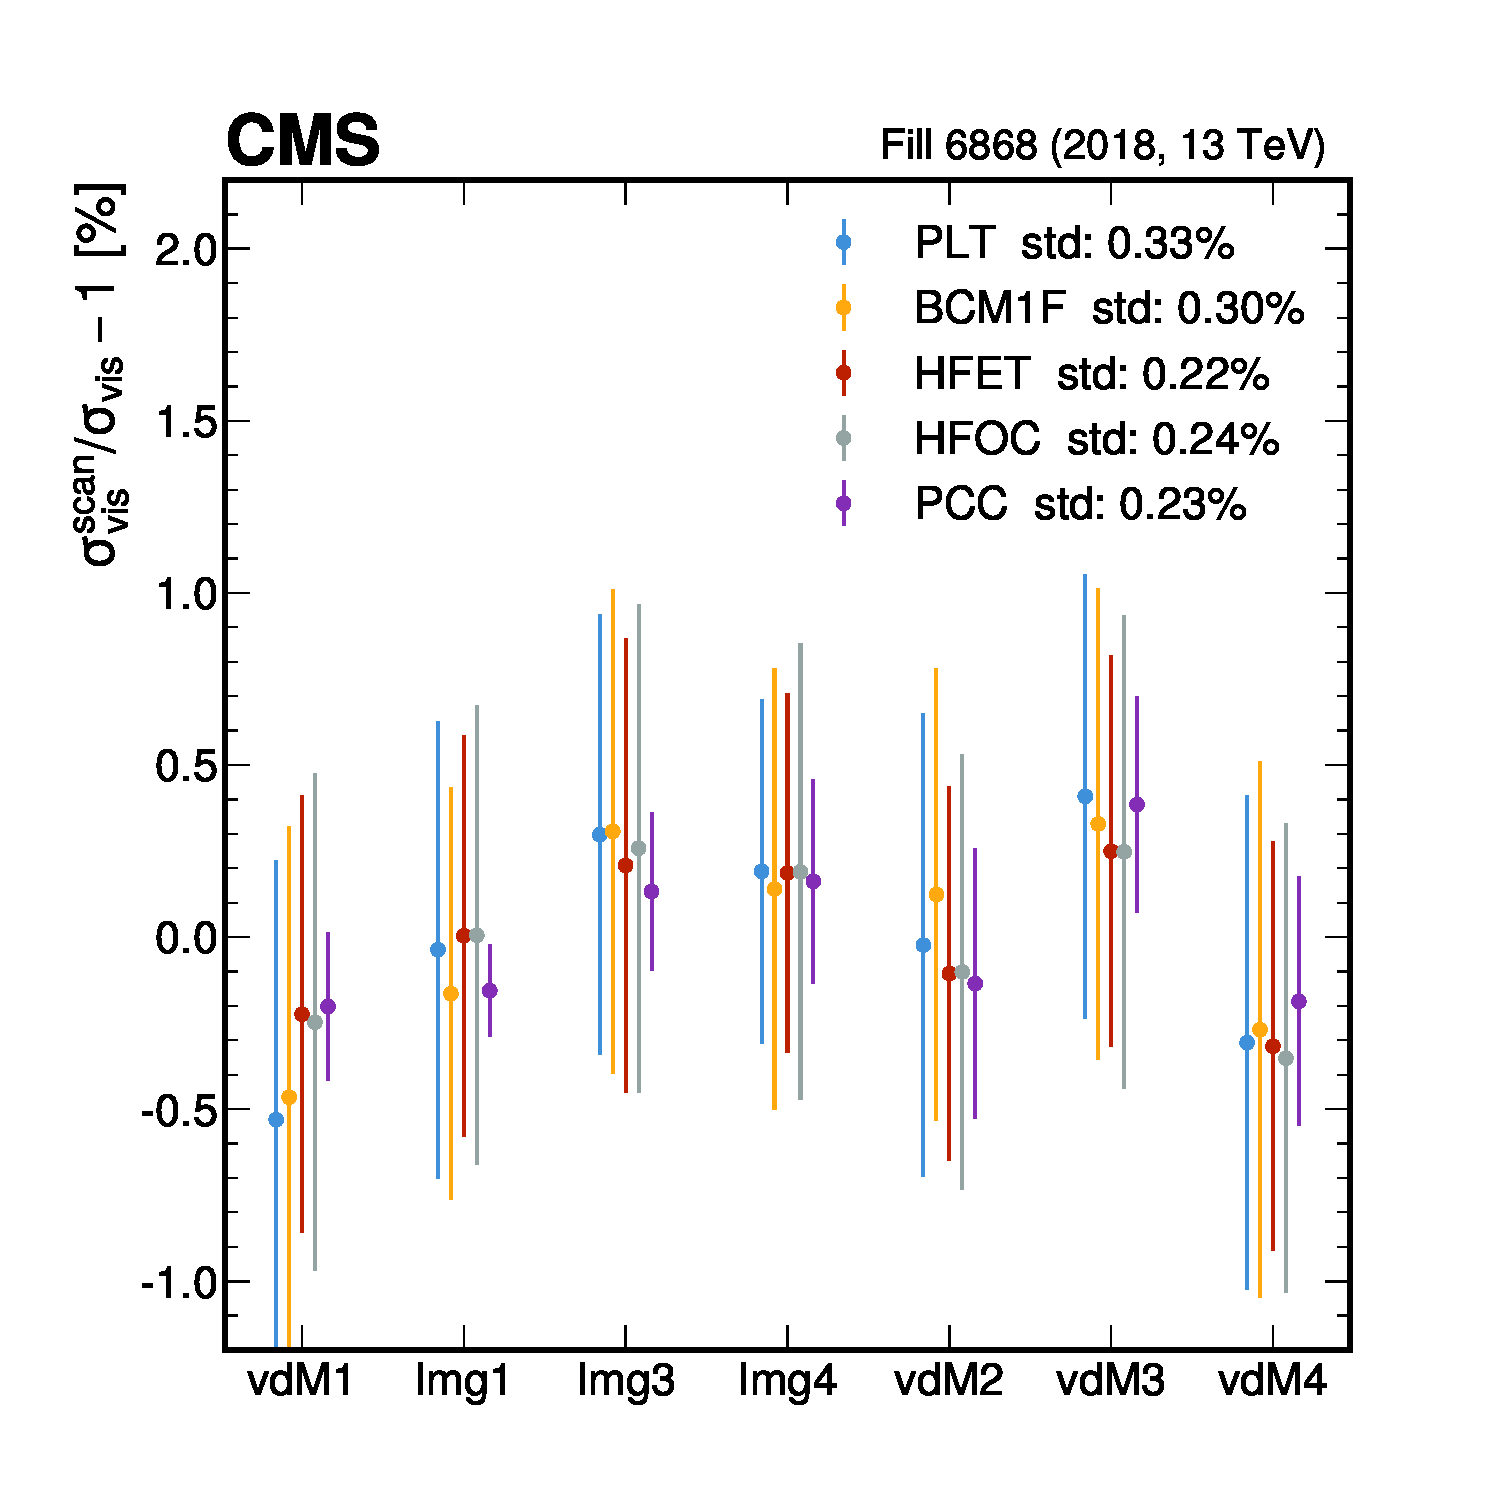
\includegraphics[width=0.49\textwidth]{figures/visible_cross_section_results/sigVisPerScanNormalized_fill6868_XY_EC.pdf}
 \caption[$\sigma_{\text{vis}}$ Stability Across Scans for All Detectors (2017 & 2018)]{The BCID averaged  $\sigma_{\text{vis}}$ divided by its average value taken over all scans for all independently calibrated detectors and all scans using the Poly4G fit function in 2017 (left) and 2018 (right). The error bars signify the standard deviation over the BCIDs. The numbers in the legend show the standard deviation over the scans.}
\label{fig:vdM_fit_sigVis_All}
\end{figure}


\section{Cross-detector comparisons in vdM Fill}


A closure test of the calibration is performed during the vdM fill by using the luminometers to measure the integrated luminosity during head-on periods. Figure~\ref{fig:vdM_xdet} illustrates the calibration consistency in the vdM fill by showing the ratio of the luminosity measured by each detector with respect to a reference. While other detectors cover a larger number of BCIDs, only five BCIDs are used to ensure compatibility with PCC data. The uncertainty is determined as the standard deviation of the measured ratio, expressed as a percentage. In 2018, BCM1F is excluded. In Figure~\ref{fig:vdM_xdet2}, the shaded area represents the standard deviation of the individual ratio averages, which defines the uncertainty assigned to the vdM calibration consistency. This uncertainty is \textbf{0.41\%} in 2017 and \textbf{0.14\%} in 2018.

\begin{figure}[!h]
\centering
  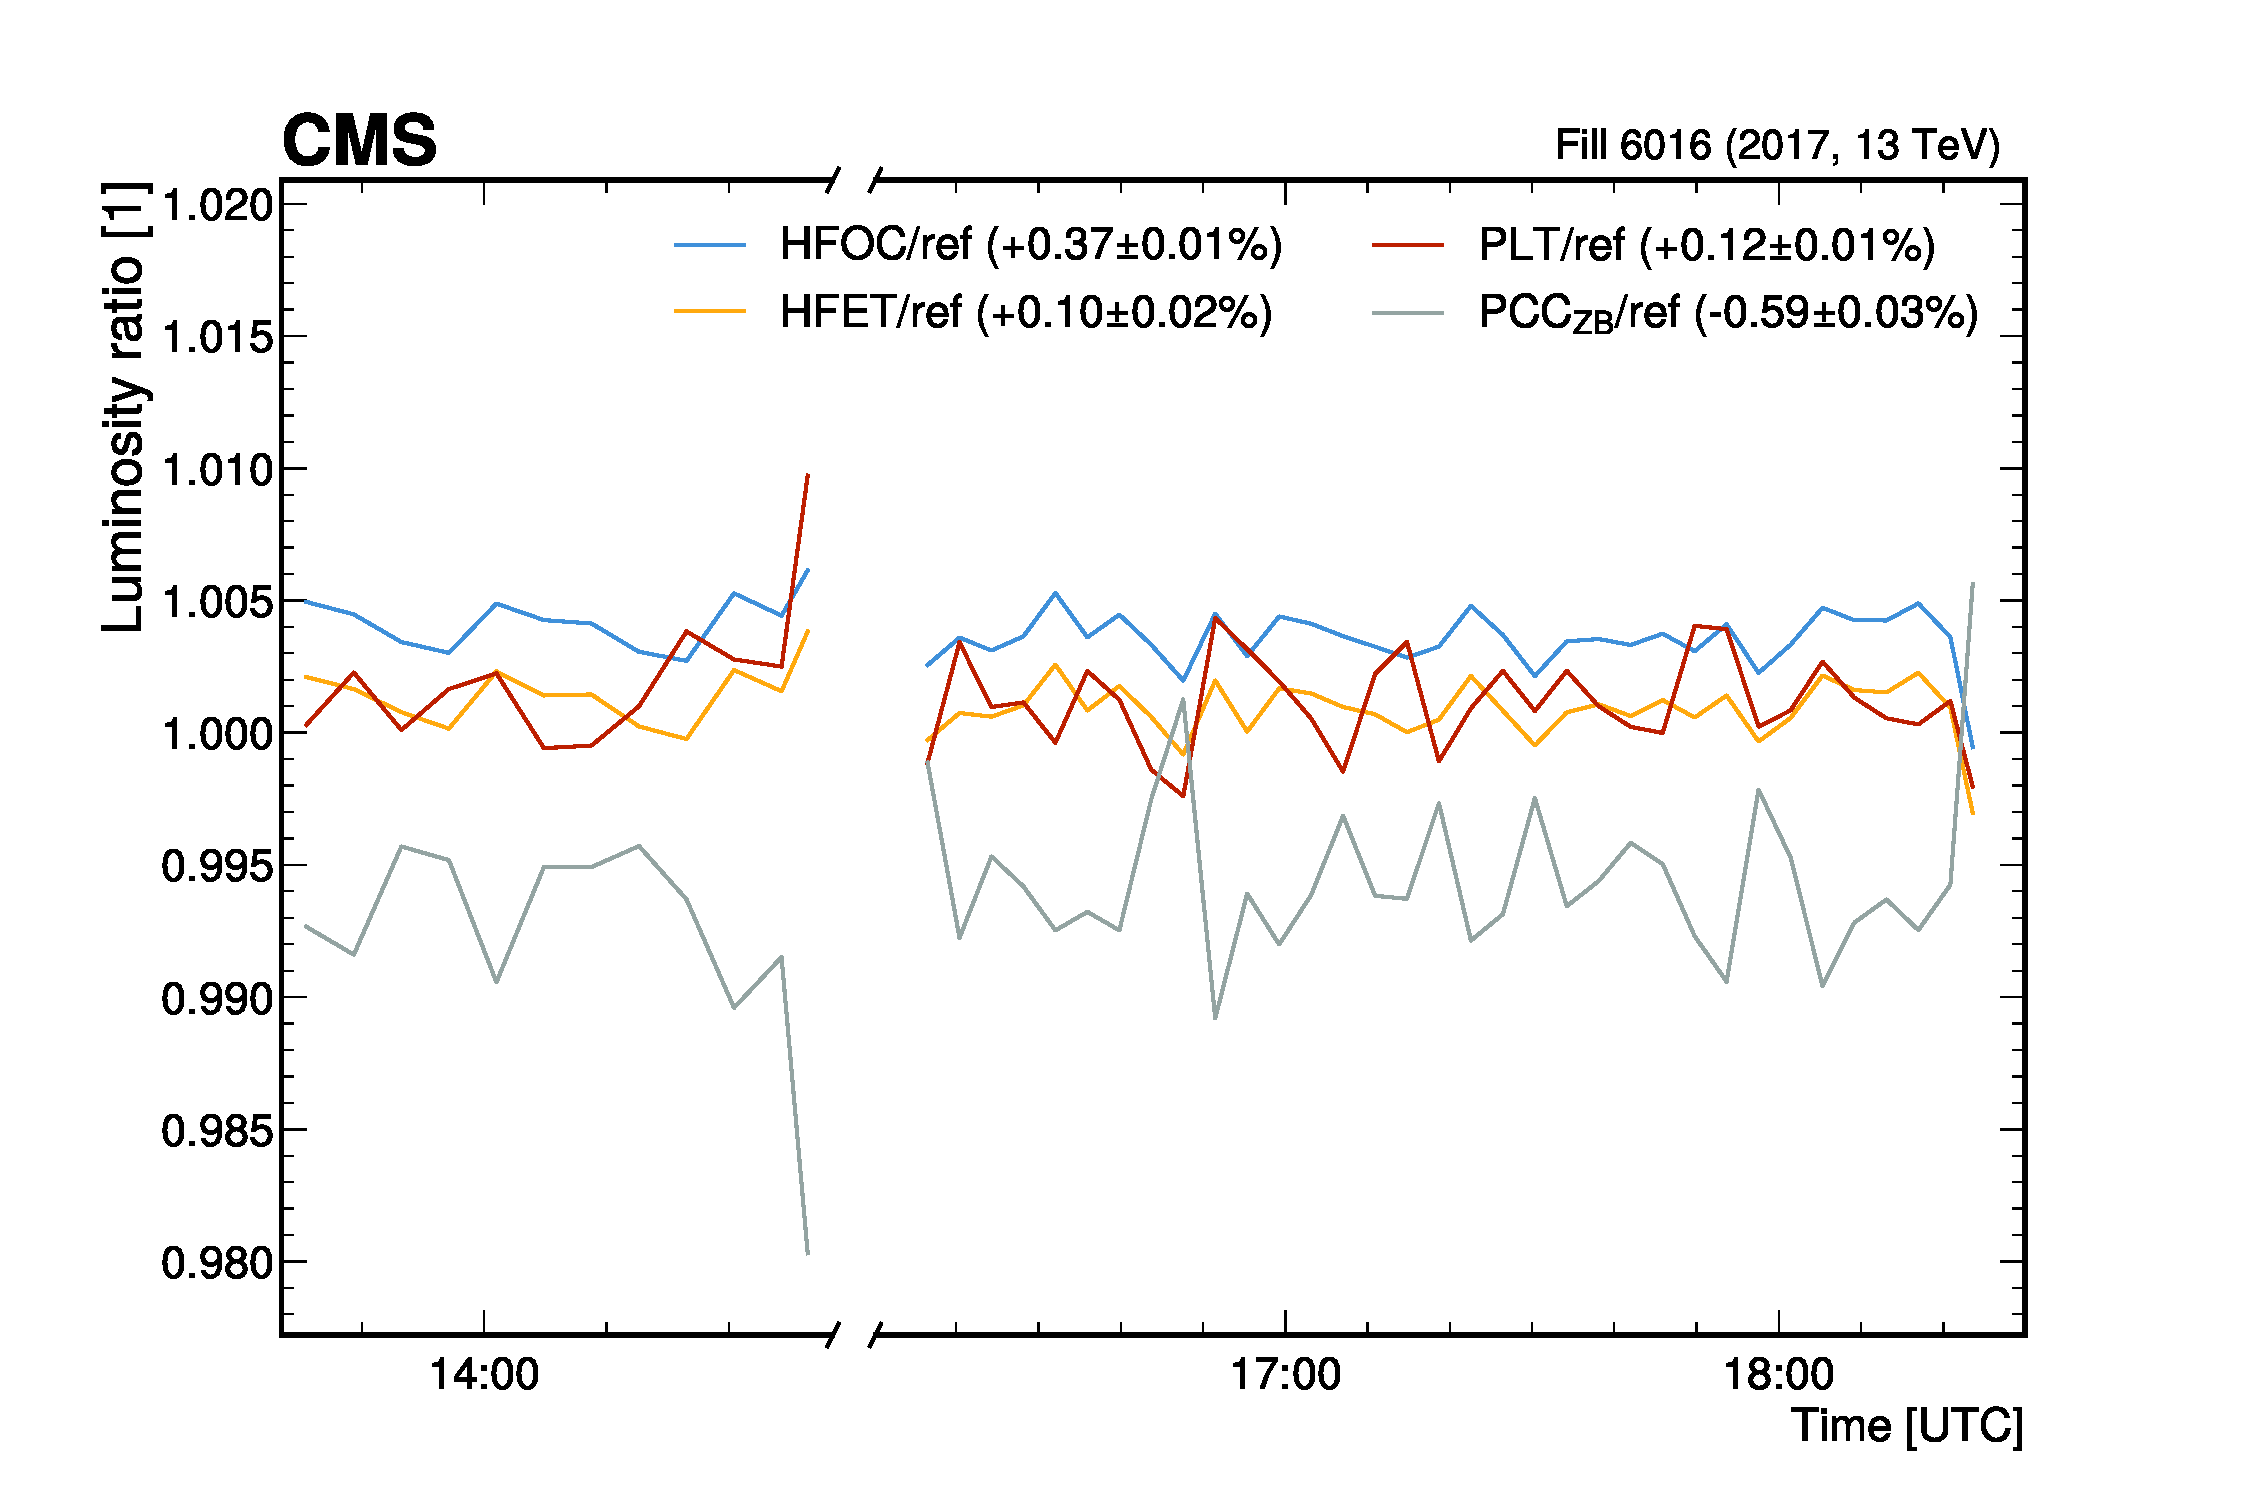
\includegraphics[width=0.49\textwidth]{figures/vdMfitting/vdMconsistency/lumi_sum5_fill6016_HFOC-HFET-PLT-PCCHD5div_HFET+HFOC+PLT+PCCHD5_ratioTrue_nls10_Xsecleg317.pdf}
  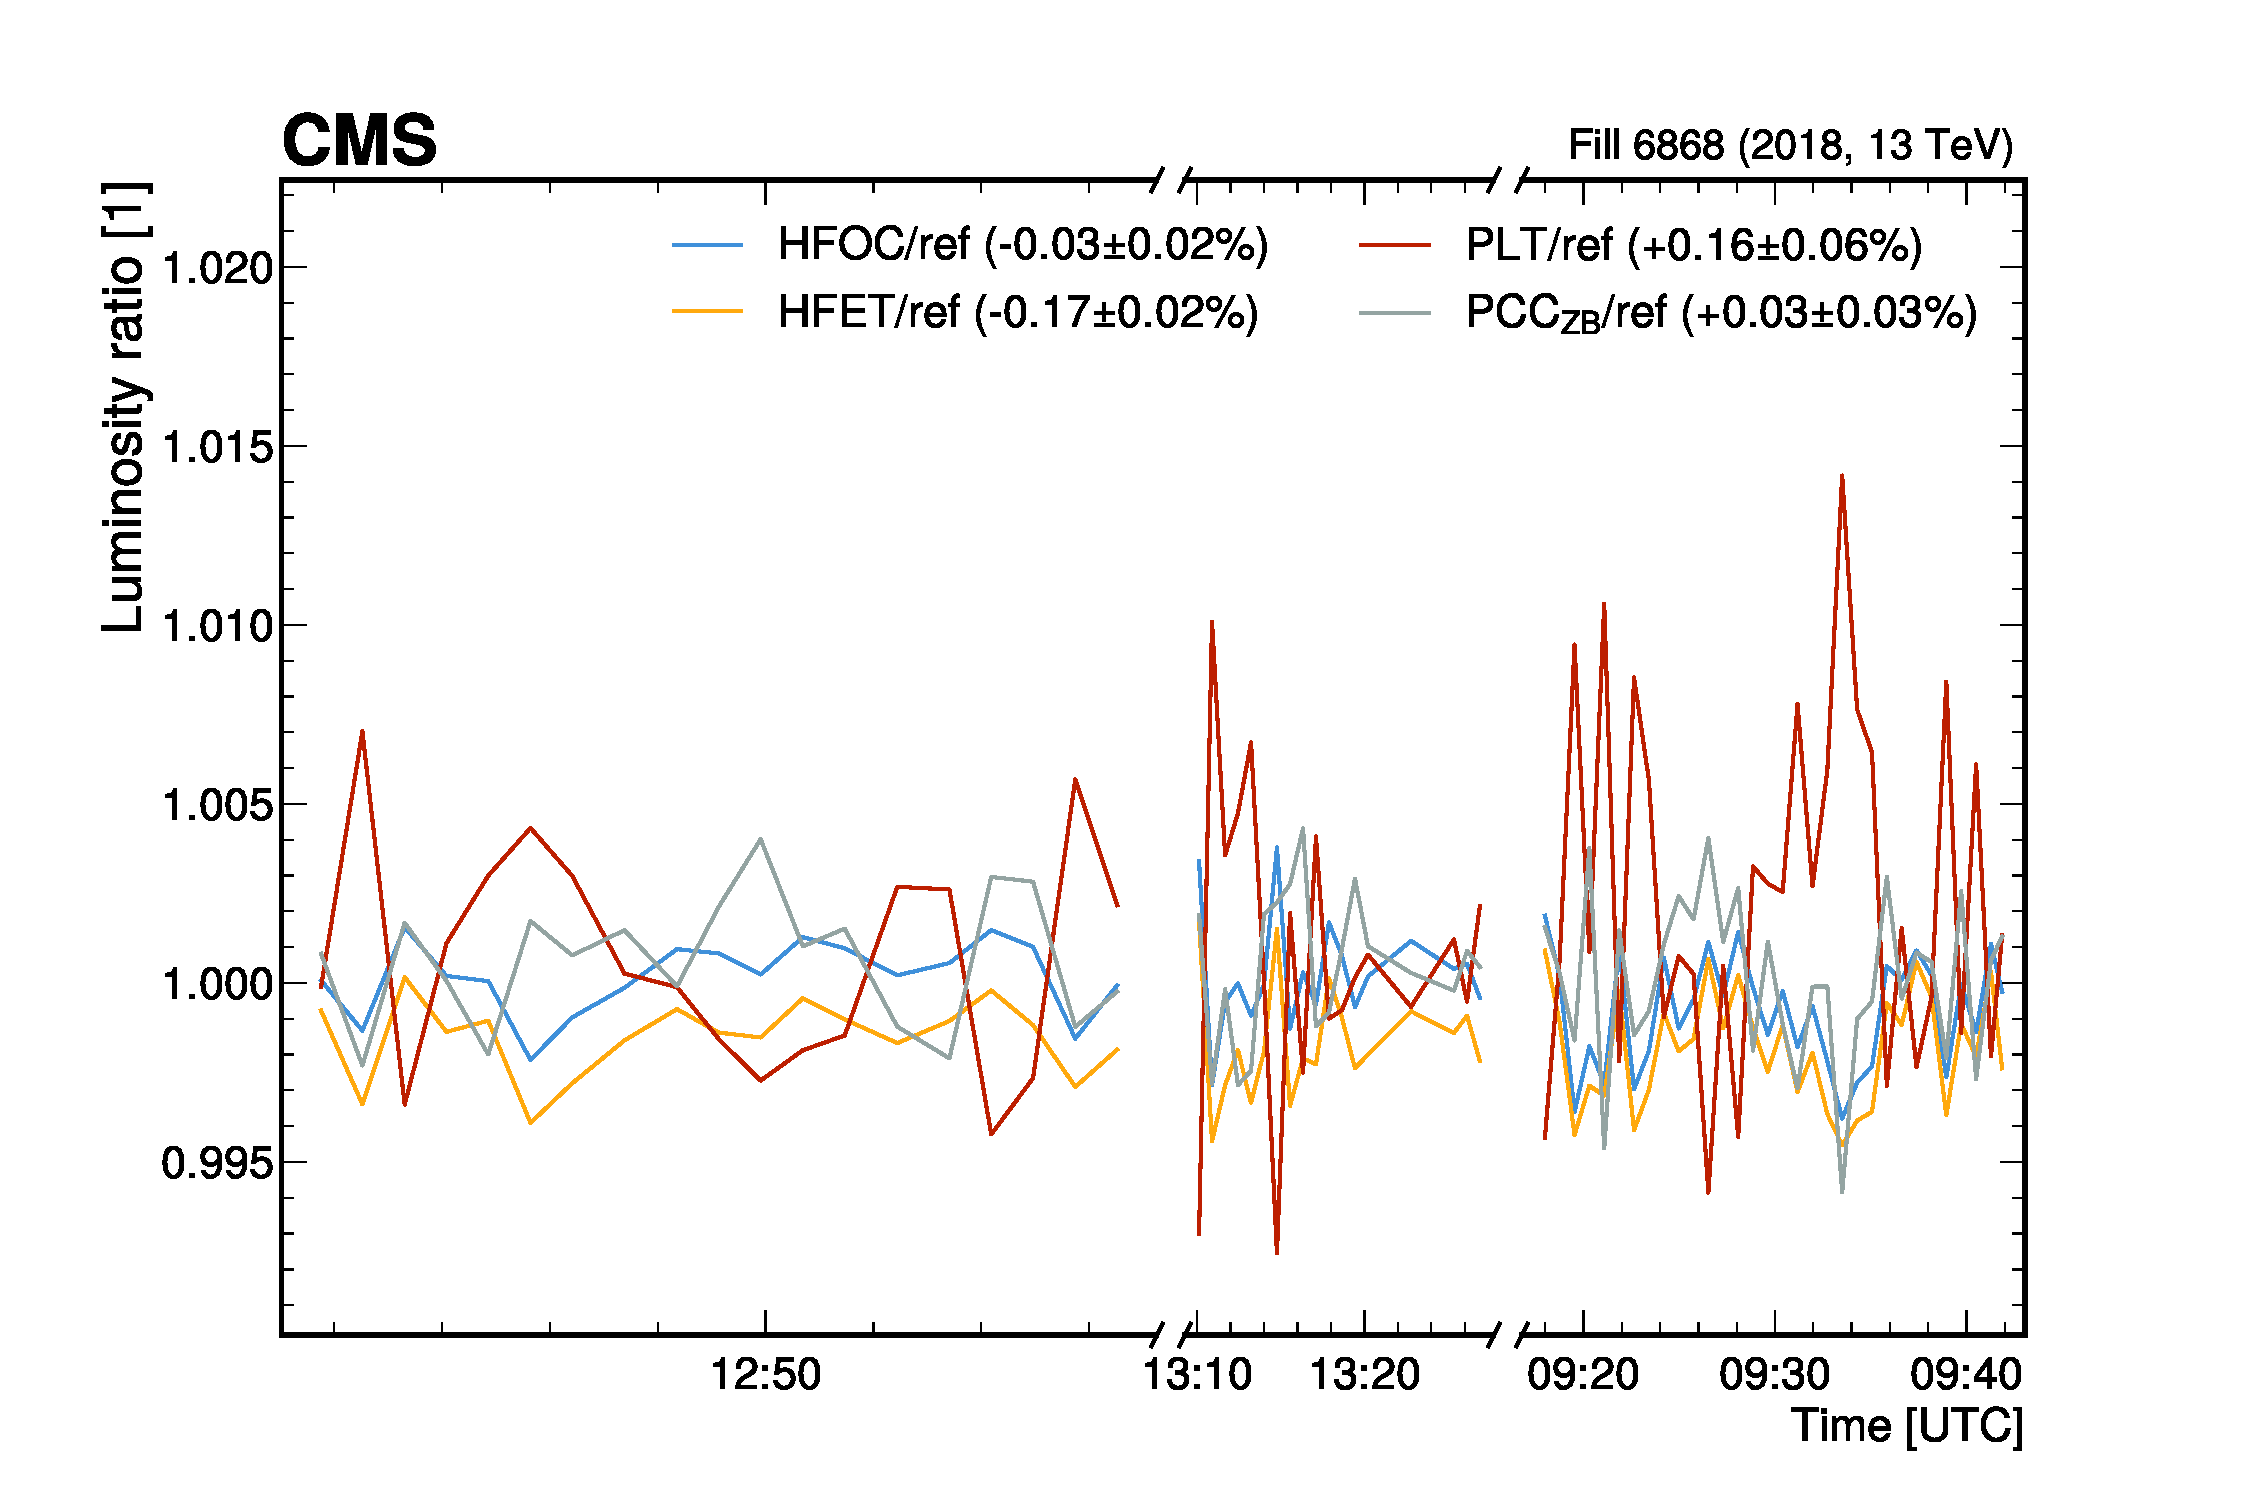
\includegraphics[width=0.49\textwidth]{figures/vdMfitting/vdMconsistency/lumi_sum5_fill6868_HFOC-HFET-PLT-PCCHD5div_HFOC+HFET+PLT+PCCHD5_ratioTrue_nls2_Xsecleg318.pdf}
 \caption[Instantaneous Luminosity Ratio with PCC Gated BCIDs (2017 & 2018)]{Instantaneous luminosity ratioin the vdM fill during head-on periods using the gated BCIDs available for PCC for 2017 (left) and 2018 (right). plot shows the values divided by a reference luminometer. The numbers in the legend signify the deviation of the integrated luminosity from the mean.}
\label{fig:vdM_xdet}
\end{figure}



\begin{figure*}[!ht]
\centering
  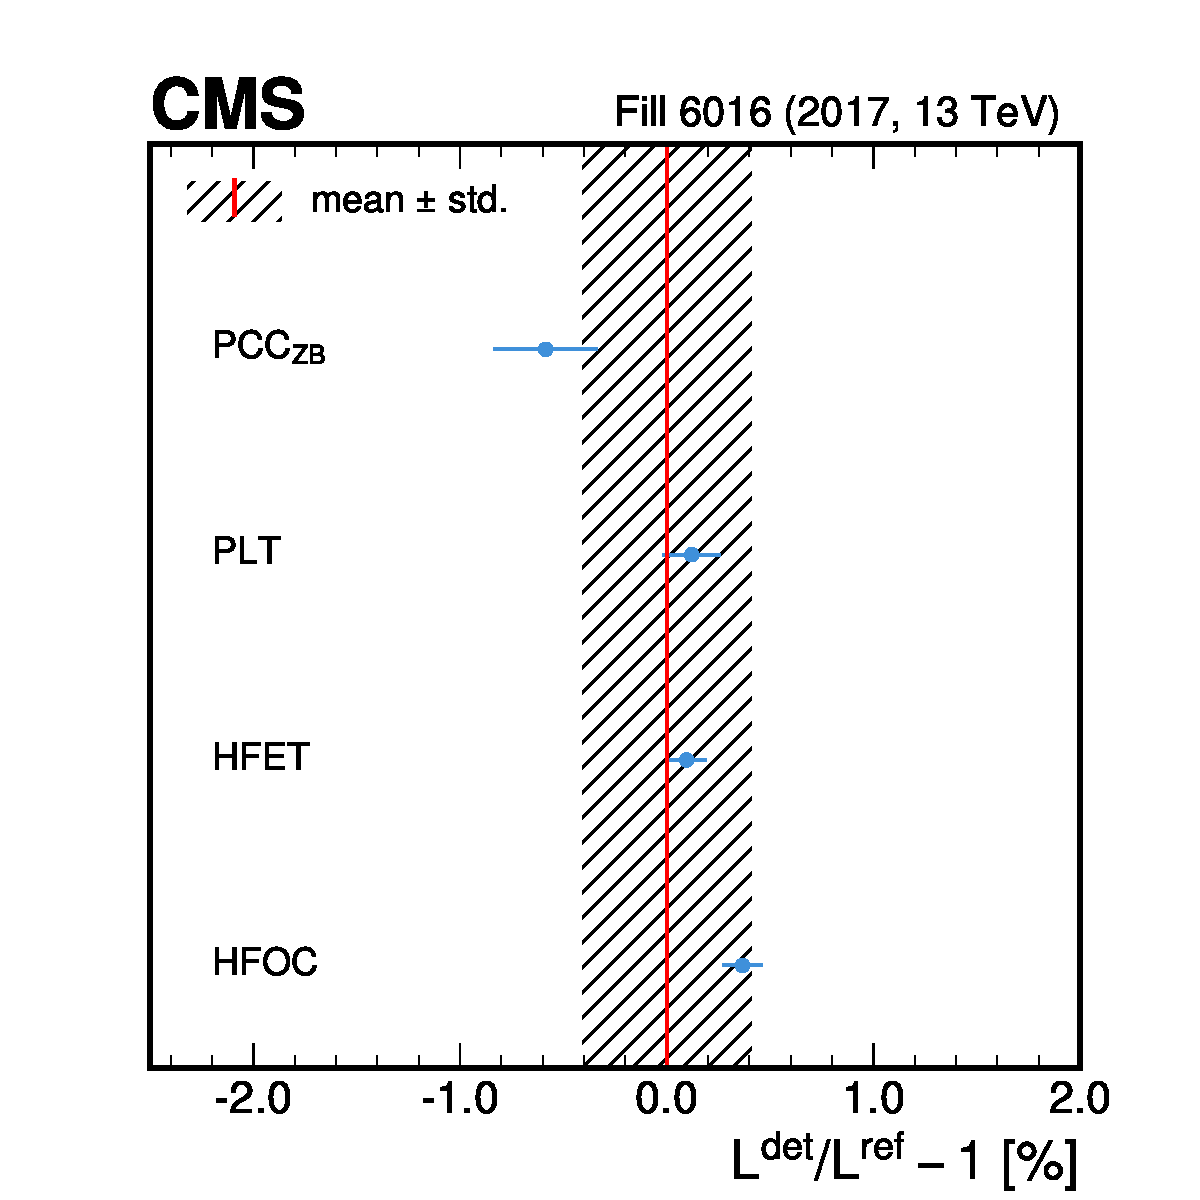
\includegraphics[width=0.49\textwidth]{figures/visible_cross_section_results/lumi_sum5_histMean_fill6016_HFOC-HFET-PLT-PCCHD5div_HFET+HFOC+PLT+PCCHD5_ratioTrue_nls10_Xsecleg317.pdf}
  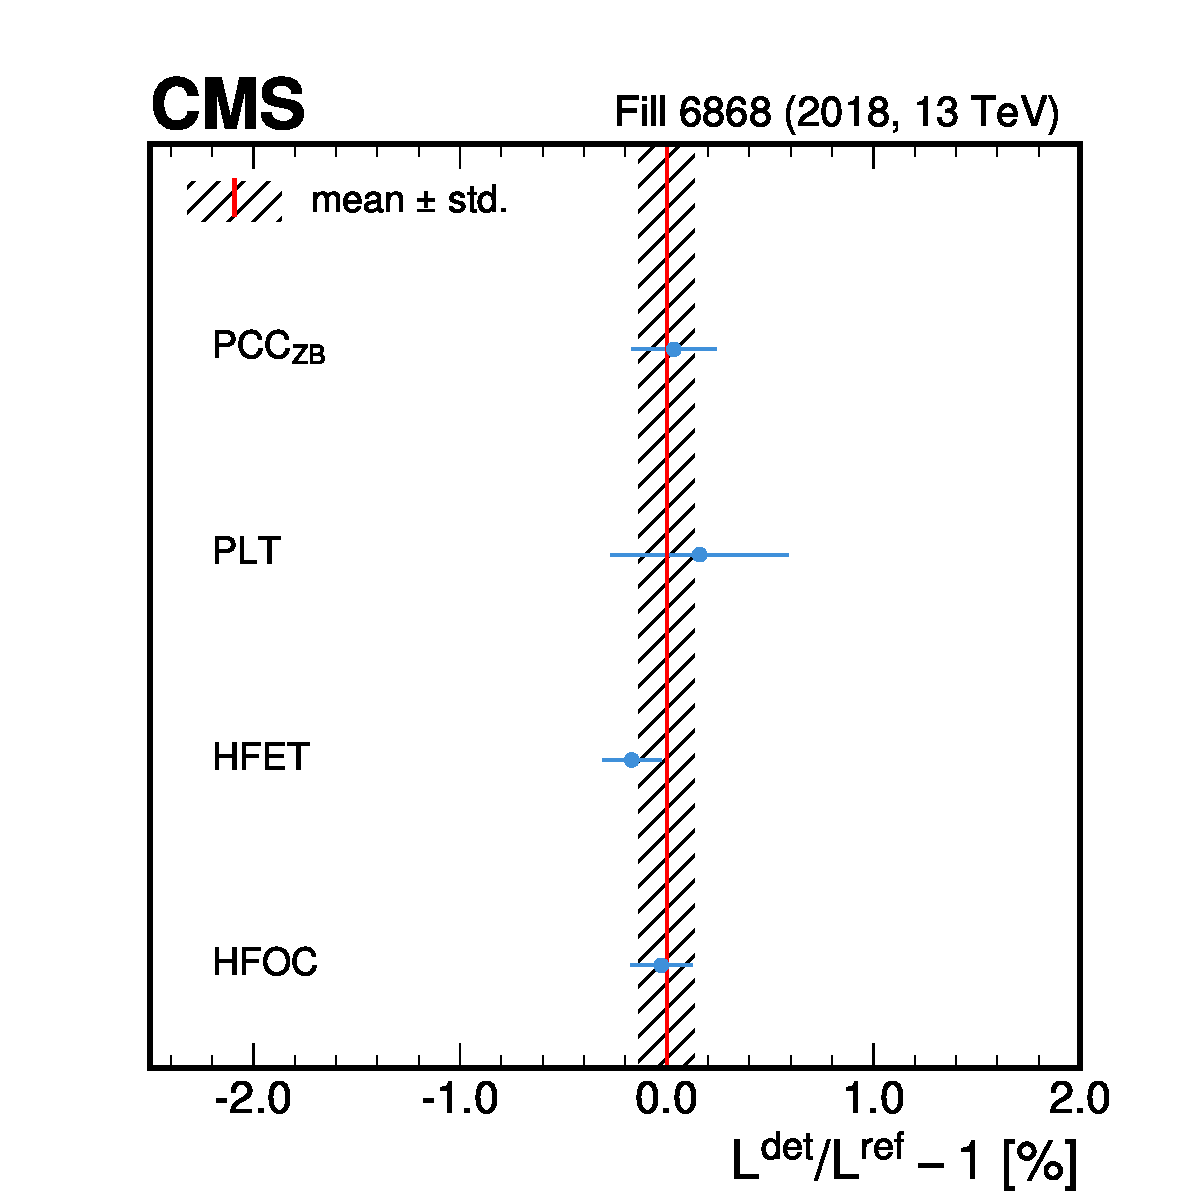
\includegraphics[width=0.49\textwidth]{figures/visible_cross_section_results/lumi_sum5_histMean_fill6868_HFOC-HFET-PLT-PCCHD5div_HFOC+HFET+PLT+PCCHD5_ratioTrue_nls2_Xsecleg318.pdf}
 \caption[Luminosity Ratios to Detector Average – vdM Head-On Periods (2017 & 2018)]{The ratios of HFET, HFOC, PLT and PCC luminosity to the detector averaged luminosity in the vdM fill for the head-on periods for 2017 (left) and 2018 (right). The points signify the average ratio, while the error bars represent the standard deviation of the ratio distribution of each of the detectors. The shaded area represents the standard deviation of the individual averages.}
\label{fig:vdM_xdet2}
\end{figure*}










\begin{comment}
\begin{table}
  \begin{center}
    \begin{tabular}{|l||c|c|} 
\hline
&  2017 [nb$^{-1}$]  &  2018 [nb$^{-1}$]  \\ \hline
BCM1F         & 4.299 &  --- \\
HFOC          & 4.331 & 1.132 \\
HFET          & 4.319 & 1.130 \\
PLT           & 4.320 & 1.134 \\
PCCHD5        & 4.289 & 1.133 \\
\hline \hline
Lumisections used & 445    &  138\\\hline
  \end{tabular}
\caption{Integrated luminosity in the head-on periods of the vdM fill using the five zero-bias gated BCIDs as measured by a set of luminometers in 2017 and 2018. }
\label{tab:vdM_xdet_intlumi}
\end{center}
\end{table}
\end{comment}






